%reflect on the headings of https://dl.acm.org/doi/pdf/10.5555/2818754.2818851 see what you can do here


%\documentclass[sigconf,review,nonacm=true]{acmart}
\RequirePackage{fix-cm}
\documentclass[]{svjour3}
\usepackage{cite} 
\usepackage{enumitem}
%\usepackage{float}
\usepackage{algorithm} 
\usepackage{algpseudocode} 
\usepackage{wrapfig} 
\usepackage{graphicx}
\usepackage{url} 
\usepackage[hidelinks]{hyperref}
\usepackage{caption}
%%%%%%%%%%%%%% 
% For reviewer responses
%%%%%%%%%%%%%%
%% Response text prefix
\usepackage{hyperref}
\usepackage[table]{xcolor}
\newif\ifblueresponse
\blueresponsetrue

 
 % Set to true for blue, false for black

\newcommand{\there}[2]{%
  \textbf{#1} \hyperlink{#1}{\textcolor{blue}{#2}} (see page \pageref{#1})%
}

\newcommand{\here}[2]{%
  \hypertarget{#1}{%
    \ifblueresponse
      \textbf{#1} \textcolor{blue}{#2}%
    \else
      #2%
    \fi
  }%
  \label{#1}%
} 

% Define the switch-on command
 

% Define the switch-on command
\newcommand{\BLUE}{%
  \begingroup
  \ifblueresponse
    \color{blue}%
  \else
    \color{black}%
  \fi
}

% Define the switch-off command
\newcommand{\BLACK}{%
  \endgroup
}




%% \BibTeX command to typeset BibTeX logo in the docs
% \AtBeginDocument{%
%   \providecommand\BibTeX{{%
%     \normalfont B\kern-0.5em{\scshape i\kern-0.25em b}\kern-0.8em\TeX}}}

%% Rights management information.  This information is sent to you
%% when you complete the rights form.  These commands have SAMPLE
%% values in them; it is your responsibility as an author to replace
%% the commands and values with those provided to you when you
%% complete the rights form.
% \setcopyright{acmlicensed}
% \copyrightyear{2018}
% \acmYear{2018}
% \acmDOI{XXXXXXX.XXXXXXX}


%%
%% Submission ID.
%% Use this when submitting an article to a sponsored event. You'll
%% receive a unique submission ID from the organizers
%% of the event, and this ID should be used as the parameter to this command.
%%\acmSubmissionID{123-A56-BU3}

%%
%% For managing citations, it is recommended to use bibliography
%% files in BibTeX format.
%%
%% You can then either use BibTeX with the ACM-Reference-Format style,
%% or BibLaTeX with the acmnumeric or acmauthoryear sytles, that include
%% support for advanced citation of software artefact from the
%% biblatex-software package, also separately available on CTAN.
%%
%% Look at the sample-*-biblatex.tex files for templates showcasing
%% the biblatex styles.
%%

% \newlist{Questions}{enumerate}{4}
% \setlist[Questions, 1]{label=RQ\arabic*., ref=RQ\arabic*}
% \setlist[Questions, 2]{label=RQ\arabic*., ref=RQ\arabic*}
% \setlist[Questions, 3]{label=RQ\arabic*., ref=RQ\arabic*}
% \setlist [Questions, 4]{label=RQ\arabic*., ref=RQ\arabic*}
%%
%% The majority of ACM publications use numbered citations and
%% references.  The command \citestyle{authoryear} switches to the
%% "author year" style.
%%
%% If you are preparing content for an event
%% sponsored by ACM SIGGRAPH, you must use the "author year" style of
%% citations and references.
%% Uncommenting
%% the next command will enable that style.
%%\citestyle{acmauthoryear}

%%
%% end of the preamble, start of the body of the document source.
\begin{document}

%%
%% The "title" command has an optional parameter,
%% allowing the author to define a "short title" to be used in page headers.

 


\title{Shaky Structures: The Wobbly World of  Causal Graphs in Software Analytics}

%%=============================================================%%
%% GivenName	-> \fnm{Joergen W.}
%% Particle	-> \spfx{van der} -> surname prefix
%% FamilyName	-> \sur{Ploeg}
%% Suffix	-> \sfx{IV}
%% \author*[1,2]{\fnm{Joergen W.} \spfx{van der} \sur{Ploeg} 
%%  \sfx{IV}}\email{iauthor@gmail.com}
%%=============================================================%%

\author{Jeremy Hulse \and Nasir U. Eisty \and
        Tim Menzies 
}

\institute{J.Hulse, T. Menzies \at
             Computer Science, NC State, USA \\ 
              \email{jphulse@ncsu.edu}   ,    
              \email{timm@ieee.org} %  \\
%             \emph{Present address:} of F. Author  %  if needed
           \and
           N. Eisty \at
           Boise State University, USA \\
            \email{nasireisty@boisestate.edu}
}


 

%%
%% The "author" command and its associated commands are used to define
%% the authors and their affiliations.
%% Of note is the shared affiliation of the first two authors, and the
%% "authornote" and "authornotemark" commands
%% used to denote shared contribution to the research.
% \author{Jeremy Hulse}
% %%\authornote{}
% %%\email{jphulse@ncsu.edu}
% %%\orcid{1234-5678-9012}
% %%\author{G.K.M. Tobin}
% %%\authornotemark[1]
% %%\email{webmaster@marysville-ohio.com}
% \affiliation{%
%   \institution{North Carolina State University}
%   \city{Raleigh}
%   \state{North Carolina}
%   \country{USA}
% }
% \email{jphulse@ncsu.edu}

% \author{Nasir U. Eisty}
% \affiliation{%
% 	   \institution{Boise State University}
% 	   \city{Boise}
% 	   \state{ID}
% 	   \country{USA}
% }
% \email{nasireisty@boisestate.edu}


% \author{Tim Menzies}
% \affiliation{%
% 	   \institution{North Carolina State University}
% 	   \city{Raleigh}
% 	   \state{North Carolina}
% 	   \country{USA}
% }
% \email{timm@ieee.org}



%%
%% By default, the full list of authors will be used in the page
%% headers. Often, this list is too long, and will overlap
%% other information printed in the page headers. This command allows
%% the author to define a more concise list
%% of authors' names for this purpose.
%%\renewcommand{\shortauthors}{Hulse, et al.}

%%
%% The abstract is a short summary of the work to be presented in the
%% article.
\date{Received: date / Accepted: date}
% The correct dates will be entered by the editor


\maketitle

\begin{abstract}
%\paragraph{}
 
Causal graphs are widely used in software engineering.
They are used to document causal relationships (and drawing conclusions and observations about the causes of events or attributes). 

Though widely used, they may also be wildly misleading.  
Causal structures generated from SE data can be highly variable.
This instability is so large that conclusions drawn from one graph
may be totally reversed in another, even when both graphs are learned from the same or very similar   project data. 
To say that another way, conclusions from causal graph generators may not generalize
since those conclusions  could be reversed   by minor changes in how those graphs are generated.

As evidence of this, this paper checks the causal graphs 
generated by four different causal graph generators (PC,FCI,GES,LiNGAM).
These generators were applied to 23  data sets relating
to three different SE tasks:
(a)~learning how software configuration options select for different system properties;
(b)~understanding how management choices effect  software projects;
and (c)~defect prediction. Graphs were compared  between (a)~different projects exploring the same task; (b)~version $i$ and $i+1$ of a system;
(c)~different 90\% samples of the data; and (d)~small variations in the     causal graph generator.
Measured in terms of the Jaccard index of the number of edges shared by two different graphs, nearly half the edges ($\frac{3}{7}\approx 0.43$) were changed by these treatments. 


Hence, before researchers can report
supposedly general conclusions from causal graphs (e.g., ``long functions cause more defects''), they should test that such conclusions hold over the numerous causal graphs that might be generated from the same data.

To allow for the repetition and/or  
refinement and/or   refutation of our results, all our scripts and data are online at \url{https://github.com/jphulse/Stability_Of_Causal_Graphs_Public}
\keywords{Empirical SE, Data Mining, Analytics }

\end{abstract}

%/Causal graphs are a type of data structure that represents causal relationships between variables in a dataset.  These graphs can be used to source problems in software systems, and potentially other systems as well.  There are various pieces of software and algorithms used to generate these graphs found in recent software engineering literature, in most of these they are used primarily with the goal of root cause analysis.  However, most of the papers discussing these algorithms and generators omit the stability of these graphs.  Generally speaking, it becomes increasingly difficult to draw conclusions from a graph produced by one of these algorithms from a given dataset if the graphs produced are not consistent.  This has the potential to make the graphs unreliable and therefore the conclusions and observations drawn from them may also be unreliable and disputable.  This in turn could decrease the value of the observations and conclusions generated based on these graphs. So I sought to find an implementation of a common algorithm to use as a baseline and run extensive experiments across various software engineering datasets. The package and implementation I found to use was the PC algorithm in the R package Pcalg TODO ADD CITATION FOR PCALG.  This is because the PC algorithm is a common baseline algorithm used in several of the generators and software I found in the other software engineering literature.  The experiments conducted involved primarily three varieties on various-sized software datasets while tuning various parameters in controlled experiments in order to observe relative stability to other trials.  The results of these experiments did reveal that there are sources of instability in the causal graphs generated by this algorithm, even when it is set to perform the "stable" variant present in the package.  The first of the three types of experiments ran included increasing alpha on a full sample of the same dataset where alpha is the significance level of the probability tests conducted by the algorithm.  The second type of experiment was to test the graphs across release to see how similar those graphs were, and to see if stability across release was observable in the graphs.  Finally, the third experiment type was to test on a random 90 percent sub-sample of the date where a tenth was left out from each graph's generation in order to observe stability when missing a random tenth of any given dataset. Both the version experiments and the significance level experiments demonstrated significant sources of instability in these graphs that were evaluated using Jaccard coefficients.
   
%%
%% The code below is generated by the tool at http://dl.acm.org/ccs.cfm.
%% Please copy and paste the code instead of the example below.
%%
% \begin{CCSXML}
% <ccs2012>
% <concept>
% <concept_id>10011007.10011006.10011072</concept_id>
% <concept_desc>Software and its engineering~Software libraries and repositories</concept_desc>
% <concept_significance>500</concept_significance>
% </concept>
% <concept>
% <concept_id>10003752.10003809.10003635</concept_id>
% <concept_desc>Theory of computation~Graph algorithms analysis</concept_desc>
% <concept_significance>500</concept_significance>
% </concept>
% <concept>
% <concept_id>10002950.10003624.10003633</concept_id>
% <concept_desc>Mathematics of computing~Graph theory</concept_desc>
% <concept_significance>500</concept_significance>
% </concept>
% </ccs2012>
% \end{CCSXML}

% \ccsdesc[500]{Software and its engineering~Software libraries and repositories}
% \ccsdesc[500]{Theory of computation~Graph algorithms analysis}
% \ccsdesc[500]{Mathematics of computing~Graph theory}



%%
%% Keywords. The author(s) should pick words that accurately describe
%% the work being presented. Separate the keywords with commas.

 
%%
%% This command processes the author and affiliation and title
%% information and builds the first part of the formatted document.



\section{Introduction}

Business users often demand explainable representations of their knowledge. For that purpose, certain representations may be deprecated  (e.g., neural nets, ensembles of decision trees) while other representations may be more popular. For example, Nader et al.~\cite{Poshyvanyk24} use causal graphs to show programmers the major relationships in their code data and then make conclusions on the best ways to effect change in that domain.  

This paper argues that such reports using causal graphs can be very misleading.  
    As an example of this problem,
 Figure~\ref{cause1}.a and Figure~\ref{cause1}.b show many differences  in the causal graphs from two different releases of the same software project:
 \begin{itemize}
     \item 
  Figure~\ref{cause1}.b tells us that {\em loc} (lines of code) causes {\em bugs}. This seems to be a reasonable conclusion (justification:   the more lines of code, the more likely a programmer will make a mistake).
  \item  
      But  Figure~\ref{cause1}.a, which is from an earlier version of the same project, offers the reversed causal connection. In this graph, {\em bugs} cause changes to {\em rfc} (how many methods wake up when a message arrives at a class)  which, in turn, causes changes to {\em loc}. 
      \item  To say that another way, in one release, lines of code seems to {\em cause} bugs
 but in another, lines of code are the {\em consequence} of bugs (this is such a  very strange result that the conclusion
 of this paper will be to not trust  this data).
      \end{itemize}
Why are causal graphs so unstable? One explanation is that the heuristics used to generate these graphs are stochastic; i.e. if we generate them twice, we can get different graphs. Hence, such graphs can hardly be considered canonical. But whatever the reason, the consequences are the same: we must doubt the generality of conclusions from causal graphs. We claim:
  \begin{quote} {\em Causal graphs generated from SE data
    may not be canonical representations of knowledge. Rather, they approximate heuristic representations that can prompt discussion but should not be used to assert definitive, generalizable conclusions.}
    \end{quote}  
To defend this value and veracity of this claim, this paper does two things. Firstly, 
our background section makes the case that causality is a widely used concept in SE.  
Secondly, experimentally, we explore casual graph instability within the static code
attributes of six open-source JAVA projects.

\here{c1}{This response will be blue.}



\there{c1}{Back to blue responses.}

\begin{figure}
\begin{center}\small
{\bf Figure \ref{cause1}.a}: In this
causal graph from Ant Version 1.5,       ``bug''s,   cause ``loc'' (see left-hand-side).
\vspace{4mm}


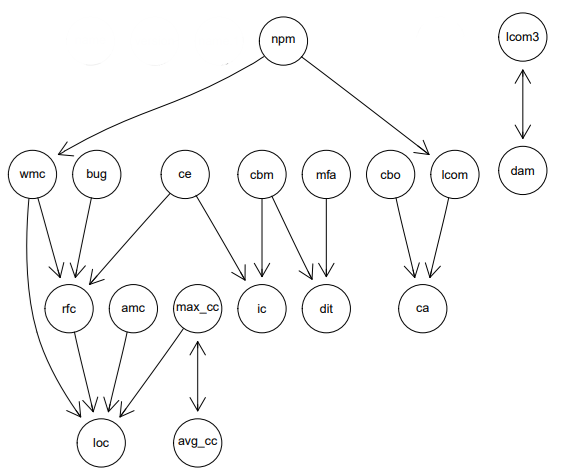
\includegraphics[width=10cm]{images/ANT_1.5_Graph.png}

\vspace{4mm}
 
{\bf Figure \ref{cause1}.b}: In this causal graph from  Ant Version 1.7, ``loc'' causes ``bug''s (see bottom-left).

\vspace{4mm}

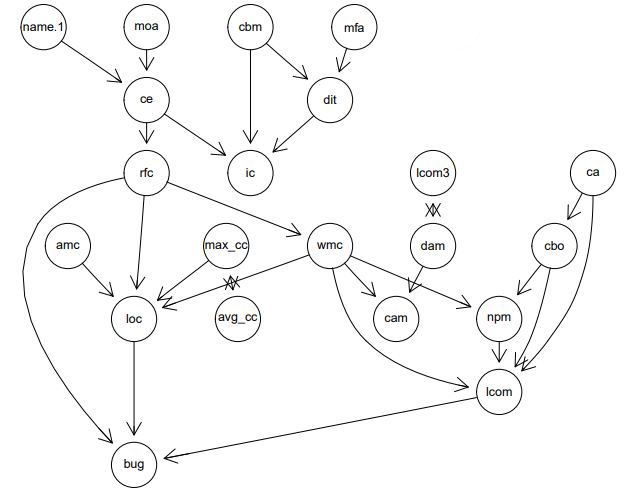
\includegraphics[width=10cm]{images/ANT_1.7_Graph.png}
\vspace{4mm}
\end{center}
\caption{Two (very different) causal graphs generated by the R pcalg package  (using \(\alpha = .01\)). For an explanation of the terms used in this figure, see Table~\ref{words}.}\label{cause1}
\end{figure} 
To structure that demonstration, we ask four research questions:
\begin{itemize}
    \item 
   {\bf RQ1:} {\em  Do the graphs  demonstrate intra-project stability across different
    releases? }
   In our corpus, over half the causal effects found in release $i$ are missing in release $i+1$.
    \item   
    {\bf RQ2:} {\em Do the graphs demonstrate inter-project stability across different projects? }
       In our corpus, over two-thirds of the casual connections present in one project
       may be different in another.  
      \item  
    {\bf RQ3:} {\em Does parameter tuning affect stability?} In our corpus, seemingly innocuous changes to tuning parameters can generate radically different causal graphs.
       \item 
     {\bf RQ4:}  {\em  How much do causal graphs change if we remove only small fractions
     of the training data?} Removing as little as 10\% of training data can lead to very
     different graphs.  
\end{itemize}
\begin{table}
\begin{tabular}{|l|p{10.65cm}|} % Adjust the 8cm as needed
\hline
\textbf{Attribute} & \textbf{Description} \\ \hline
name & The name of the software project \\ \hline
version & The version of the software project \\ \hline
name.1 & The extended name of the full software package (if one exists) \\ \hline
wmc & Weight Method Class or McCabe's complexity: Branch instructions in a class. \\ \hline
dit & Depth Inheritance Tree: Counts the number of ``fathers" a class has. \\ \hline
noc & Number of Children: Counts the number of immediate subclasses. \\ \hline
cbo & Coupling between objects: Counts the number of dependencies a class has. \\ \hline
rfc & Response for a Class: Counts unique method invocations in a class. \\ \hline
lcom & Lack of Cohesion of Methods: Calculates LCOM metric. \\ \hline
ca & Afferent Couplings that counts the  classes that depend on a given class. \\ \hline
ce & Efferent couplings: counts the number of classes that a given class depends on\\ \hline
npm & Number of Public methods: counts of the number of public methods. \\ \hline
lcom3 & LCOM* (Lack of Cohesion of Methods): Modified version of LCOM. \\ \hline
loc & Lines of code: Counts the lines of code, ignoring empty lines and comments. \\ \hline
dam & Data Access Metric is the ratio of the number of private attributes to the total number of attributes declared in the
class. \\ \hline
moa & Measure of Aggregation. Counts the number of data declarations (like class-level variables) whose types are user-defined classes.\\ \hline
mfa & Measure of Functional Abstraction. Ratio of inherited methods to all methods. \\ \hline
cam & Cohesion Among Methods of Class that measures the similarity of parameter lists of methods in a class, indicating method cohesion.\\ \hline
ic & Inheritance Coupling that counts the number of parent classes to which a class is coupled. It indicates the class's dependency on inherited methods.\\ \hline
cbm & Coupling Between Methods - measures total complexity of coupling between class methods.\\ \hline
amc & Average Method Complexity -   the average complexity of methods in a class. \\ \hline
max\_cc & Maximum Cyclomatic Complexity -   max. cyclomatic complexity among the methods of a class. \\ \hline
avg\_cc & Average Cyclomatic Complexity- calculation of the average cyclomatic complexity of methods in a class. \\ \hline
bug & Number of bugs \\ \hline
\end{tabular}
\caption{Variables see in Figure~\ref{cause1}.}\label{words}
\end{table}

Note that we do not show that {\em all} causal graphs are unstable for {\em all} kinds of data analytics. That would be beyond the scope of any one paper. However, what our literature review will show is that issues of causal graph instability are rarely discussed in the SE literature. This means that prior generalizations based on causal graphs now have an extra threat to validity, i.e., that their results may not hold across even minor variations to the training methods. 

 Overall, the contribution of this paper is to document the   frequency and impact  of the SE causal graph instability problem: 
   \begin{itemize}
       \item
        {\em Frequency:}  
      The instabilities of Figure~\ref{cause1} are not just a quirk of one data set.
         Rather, these instabilities are rampant across multiple data sets and multiple sub-samplings and tunings of the causal graph generation process.
         \item {\em Impact:} Our experiments explore very small changes to the training method (e.g. {\bf RQ4}). Yet even those small changes result in very different graphs.  
         \item Further, we document this impact and frequency in a repeatable and refutable
         manner. All our scripts and data are freely available online\footnote{ {\url{https://github.com/jphulse/Stability_Of_Causal_Graphs_Public}}}  thus allowing
         others to repeat/ refine/ or even refute our claims.
     \end{itemize}
These are important contributions.    As shown in \S\ref{cinse},   (a)~there is a growing interest in causality in SE, yet (b)~there is often a lack of attention to the stability of causal graphs~\cite{gamella2020active}. 
Stability checks, such as running multiple iterations with different random number seeds, are crucial for ensuring the robustness and reliability of the inferred causal relationships~\cite{elwert2013graphical}. 
However, this practice is frequently overlooked, which leads to questionable or unreliable conclusions.

 
 


% To demonstrate this problem,  we set ourselves the question: 
% \begin{quote} {\em If we were a  SE researcher trying to make causal inferences, what tools would we select and how stable are the conclusions from those tools?}
% \end{quote}
% This paper shows that for at least one  family of causal graphs generators,
% which might be selected by an SE researchers, those generators lead to unstable conclusions about defect prediction. 
%   More specifically:
%   \begin{itemize}
%       \item  SE papers often train models from release $i$ then test on release $i+1$. Worryingly, we show  that this kind of {\em intra-project variation} causes very large causal graph changes.  
%   \item 
%  SE paper often offers comments across multiple projects. We find that even in similar domains, and even with data sets with the same structure (column names), the causal graphs seen in this {\em  inter-project variation}  are wildly
% different.
%     \item Other large-scale variations in the graphs were seen
%     in the intra-project case when the tuning parameters of the causal graph were changed. These suggests that these causal graphs may be, in part,
%     hallucinations induced by some random choice of parameters within the causal
%     graph generator.
% \end{itemize}   


 
 

  
      
% \subsection{When Instability Does not Matter}\label{relax}

% Having shown an example where instability
% causes problems, there are also   SE applications where  that  instability  may not matter. 

% For example, when debugging software, we seek clues as to where to look for errors. In that search it can be useful to have an assistant that points out where errors might be found. That assistant needs not offer generalizable conclusions. Rather, that assistant can be useful even it offers multiple suggestions (just as long as most of its suggestions takes us to places where it is more likely to find the cause of a crash).
% Hence, for applications that involving generating (and perhaps even prioritizing) candidate solutions, the indeterminacy of causal graph generation might actually be a feature, not a bug. 


% That said, even when debugging, ins as we will show, 

 The rest of this paper is structured as follows:
 \begin{itemize}
 \item \S\ref{back} argues causal graph instability in SE is potentially a problem since
such graphs are widely used in SE.   
That section discusses some causal theories and algorithms. After that,
it discusses the widespread use of causality
and causal graphs.
\item  \S\ref{xp}  documents the extent of the causal graph instability problem via some controlled experiments on SE data.
\item {\S}\ref{discuss} discusses the validity of our conclusions and possible future work.
\end{itemize}




  
\section{Background } \label{back}







\subsection{Causality}

In 1973, David Lewis~\cite{Lewis1973} said, ``causation is something that makes a difference, and the difference it makes must be a difference from what would have happened without it''; i.e.
$T$ ``causes'' $Y$ if changing $T$ leads to a change in $Y$, keeping everything else constant. 


 Proponents of causality argue that it is a more informative concept than mere correlation. If we say that two variables X, Y are correlated, then this leaves open  many questions:  
 \begin{itemize}
     \item Does X cause Y?
     \item Does Y cause X?
     \item Is there some third hidden confounding variable that actually 
     is the cause of X and Y?
 \end{itemize}
 On the other hand, when we can say X causes Y, we can move from merely observing the world to actually changing it. Nadir et al. call this ``climbing Pearl's Ladder of Causation''~\cite{Poshyvanyk24}.  Judea Pearl was an early pioneer in causality in AI.  In his seminal textbook with  Mackenzie~\cite{pearl2018book},  Pearl said that causal inference explores   questions of association (what is?),
counterfactual interventions (what if?), and pure counterfactuals (why?). Different levels of human cognitive styles, says Pearl, match different levels of this hierarchy. For example, merely reporting ``what is?'' via correlation
(or some method that infers $y=f(x)$) is level one.
Deciding ``what to do?''  (i.e. what interventions to take) is a higher-level task that is more cognitively difficult. This requires questions about ``what if?'' and ``what if I do X?''.  
Finally, above  the ``doing'' level is the ``imagining'' level that explores
issues of ``why?'' and ``was it X that caused Y?'' and ``what if I had acted differently?''. 

Causal graphs are a data structure that aims to showcase causal relationships between a set of random variables.
Causal graphs, also known as a causal diagram (and perhaps a causal Bayesian network), is a graphical representation used to illustrate and analyze the causal relationships between variables in a system~\cite{Pearl1995}. 

In causal graphs, nodes represent variables or events, while directed edges (arrows) indicate causal influences from one variable to another. 
Causal graphs are typically structured as Directed Acyclic Graphs (DAGs), meaning they have directed edges and no cycles, ensuring a well-defined ordering of events or variables~\cite{williams2018directed}.
Figure~\ref{cause1} showed three examples of such graphs.

 
 In these graphs, when there is an edge between any two nodes, X and Y, going from X to Y, one can imply that X has a causal effect on Y.  This is combined with asserting that given all other additional random variables in the set, there is no variable Z for which X and Y exhibit conditional independence\cite{CAUSALLDEF}\cite{PCParalell}, within a threshold.  In theory, observations can then be made from these graphs to identify variables, not just in terms of correlation to each other, but in an attempt to identify variables as cause and effect. 

 \subsection{Applciations of Causality}

 \here{E1}{This section we discuss  our assumptions behind the kinds of causal reasoning explored in this paper.  In summary, we will say 
 \begin{quote}
 {\em There are many ``right'' ways to use causality in SE and  causal structure instability can  \underline{\bf negatively impact them all}. }
 \end{quote}}


\begin{table}[t!]
    \centering
    \caption{Papers by SE field. From~\cite{nasir}.}\label{field}
    \begin{tabular}{ll}
        \hline
        \textbf{Software Engineering Fields} &  \\
        \hline
        Testing & 17 \\
        Deployment & 9 \\
        Design & 7 \\
        Development & 5 \\
        Maintenance & 5 \\
        Collaboration & 1 \\
        \hline
    \end{tabular}
\end{table}

\begin{table}[t!]
    \centering
    \caption{Papers by application in SE fields. From~\cite{nasirXXX}.}\label{apps}
    \begin{tabular}{ll}
        \hline
        \textbf{Causal Reasoning Applications} &  \\
        \hline
        Causality Graph & 17 \\
        Groundwork to Facilitate Causality & 12 \\
        Bayesian Model & 5 \\
        Granger Causality Test & 3 \\
        Difference-in-Differences Model & 2 \\
        Counterfactual Prediction & 2 \\
        Statistical Analysis & 1 \\
        Evidential Network & 1 \\
        Propensity Model & 1 \\
        \hline
    \end{tabular}
\end{table}

 \BLUE Our reading of the literature is that causal graphs are becoming more popular in SE. Hence we must expect that any list of their application area (e.g. Table~\ref{field} and \ref{apps})
will soon be out-dated. This is to say that any discussion on how to use them and   the ``right''
way to apply them must be generalized beyond their current appreciations areas (so those applications areas are rapidly changing).  

 

We  have seen that causal inquiries in software engineering can take many forms including:\begin{enumerate}
  \item
  Confirmatory studies;
  \item
  Generative studies;
  \item
  and Exploratory patching.
  \end{enumerate}
  {\em Confirmatory studies} begin with established assumptions (often visualized as causal graphs), which are then tested. While useful, relying solely on confirmatory analysis risks missing novel insights and introducing bias. The Wikipedia page "List of discoveries influenced by chance circumstances"\footnote{ That list includes pacemakers, microwave ovens, vulcanized rubber, penicillin,     Big Bang radiation, the Michelson-Morley effect, viagra, saccharin, etc}    and Breiman's "Two Cultures" paper~\cite{breiman2001statistical} highlight the limitations of restricting analysis to expected outcomes. Furthermore, for confirmatory studies, reviewers may question the ground truth of manually generated causal graphs\footnote{Recently we had a confirmatory causality paper rejected from a senior SE conference. In that work, to test out some causal algorithms, we compared causal graphics that were (a)~generated automatically or (b)~generated manually (by a dozen   SE Ph.D. students drawing   graphs denoting their  proposed causal relations between  software project attributes). Reviewers rejected the work saying that the   analysis could be misdirected since it made the incorrect assumption  that these dozen graphs were a trustworthy ground truth. }. 

 {\em Generative studies}, conversely, start without pre-existing assumptions, generating causal graphs that are then examined for insights. However, this approach can yield absurd conclusions, such as the incorrect assertion that bugs cause lines of code, or spurious correlations like the (in)famous relationship reported  between chocolate consumption  per 10 million persons and Nobel laureates per country~\cite{messerli2012chocolate}\footnote{In that satirical article,
 Messerli~\cite{messerli2012chocolate} reports that chocolate consumption correlates to   Nobel prices at $r=0.79, P<0.0001$.}.

  
 \begin{wrapfigure}{r}{1.5in}
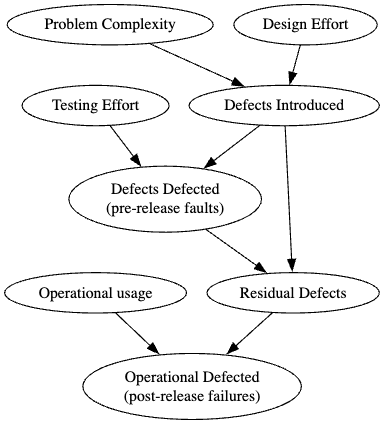
\includegraphics[width=1.5in]{fenton.png}
\caption{    Fenton \& Neil~\cite{Fenton2000SoftwareMR} expand Equation~\ref{ff} into this model. }\label{fenton}
\end{wrapfigure} 
~{\em Exploratory  patching} (a.k.a. ``making it up as you go along'')  means altering  causal models based on unexpected findings. 
For example, while working on   software faults and failures.
Fenton \& Neil challenged the  traditional causal view that
\begin{equation}\label{ff}
\mathit{faults} \rightarrow \mahthit{failures}
\end{equation}
by presenting data showing systems with few pre-release faults but
many post-release. To reconcile this anomaly, they expanded the traditional  causal model, incorporating factors like system usage, defect detection, and design effort. This revised model show how (e.g.) systems with no testing could exhibit few faults but many failures
(see Figure~\ref{fenton}). Even though this extended causal model lacked empirical validation, it was still accepted by reviewers at top SE venues~\cite{fenton1999critique,Fenton2000SoftwareMR}.


Making it up as you go along
when used unwisely,   can   certify incorrect models.  
The key, says SE methodology guru Ernst~\cite{Ernst2023}, is to  distinguishes between what he calls
{\em confirmatory} and {\em exploratory} studies. Making it up as you go along is unacceptable in confirmatory research. But if the  
 theory update methods is pre-specified, then making it up as you go along is  permissible in exploratory research.
Methods for pre-specifying the theory revision  method include:
\begin{itemize}
\item
Data mining~\cite{witten2002data}, which we take to mean a batch creation/update
of a model using numerous examples. 
\item Active learners~\cite{senthilkumar2024largelanguagemodelsimprove}, which make up a  a new theory every time a new example is sample.  Active learners querying the theory built so far to find the next most informative example to sample. After each new sample, the active learner makes up a new model using all the examples labelled thus far.
\item 
The Fenton \& Neil approach described above  that generated causal models, identified counter-examples, then extended the model accordingly. 
\end{itemize}

Regardless of whether we are doing 
confirmatory studies;
or  genarative studies
or exploratory  patching

   \BLACK

 
 
 

% \begin{wrapfigure}{r}{2.5in}
% 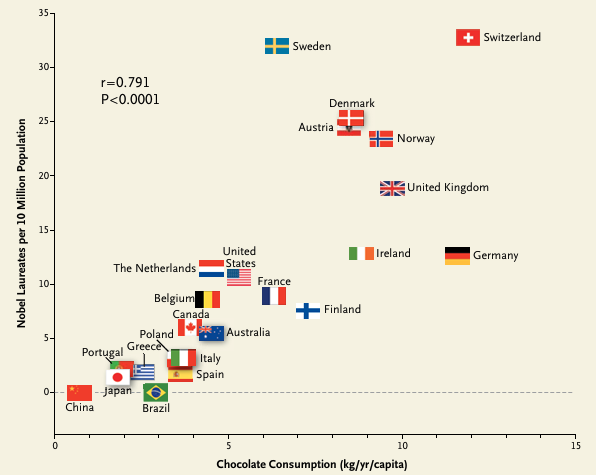
\includegraphics[width=2.5in]{chocolate.png}
% \caption{Does increased chocolate consumption cause   Nobel prizes? From~\cite{messerli2012chocolate}.}\label{chocolate}
% \end{wrapfigure}
%  On the other hand, relying just on generative analysis can result in absurd conclusions.
%  For example,
%  Figure~\ref{cause1}.a offered the absurd conclusion that   bugs causes lines of code (and not the other way around).
% For another example of an absurd conclusion,
% consider the (in)famous  Messerli's~\cite{messerli2012chocolate}    linear correlation   \mbox{($r=0.79,P<0.0001$)} between chocolate consumption per capita and the number of Nobel laureates per 10 million persons
%  (see Figure~\ref{chocolate}).    Messerli proposes an causal mechanism for this effect\footnote{ ``Improved cognitive performance with the administration of a cocoa polyphenolic extract has   been reported in aged WistarUnilever rats.''~\cite{messerli2012chocolate}} but a carefully reading of that article shows that Messerli means this more as    satire rather than a serious
%  scientific conjecture. 

%  \begin{wrapfigure}{r}{2in}
% 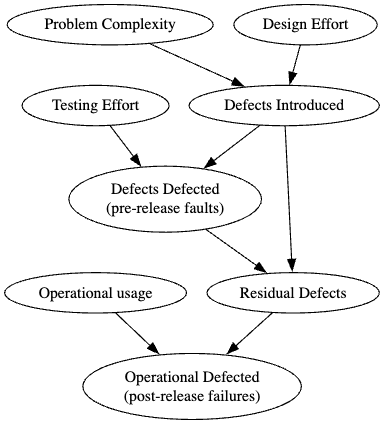
\includegraphics[width=2in]{fenton.png}
% \caption{    Fenton \& Neil~\cite{Fenton2000SoftwareMR} expand Equation~\ref{ff} into this model. }\label{fenton}
% \end{wrapfigure}
% Finally, surprise-driven causal refinement allow analysts to bias the final causal model according to their expectations, intuitions, and local data. From a traditional methodological viewpoint, it may seem strange to allow analysts to bend the theory  to their whim since     ``making it up as you go along''
% seems a recipe for sloppy science. 

% Nevertheless, there are
% documented cases where ``make it up as you go along'' causality
% has been recognized as good science.
% Consider the discussion of software faults and failures in  Fenton \& Neil~\cite{Fenton2000SoftwareMR}. 
% In reliability engineering ``faults'' are potential problems founds  during pre-release testing while ``failures'' are actual problems seen post-release.
%  Fenton \& Neil   note that the traditional causal argument in SE is that:
% \begin{equation}\label{ff}
% \mathit{faults} \rightarrow \mathit{failures}
% \end{equation}
% Fenton \& Neil  presents data from multiple projects where, 
%   systems with many faults are observed to  have few failures (and vice versa).
%  Given the   causal model of Equation~\ref{ff}, this 
%  data is in inexpiable.

% Fenton \& Neil fix this anomaly by elaborating on their causal models (see Figure~\ref{fenton}).
% Operational  failures, they argue,  are a product of how much the system is used and how many defects are left over by development. This, in turn, is a product of how many defects are introduced and defected (as faults). Furthermore, defects are introduced by either high problem complexity and/or low design effort. Lastly, defects are only detected by testing effort. This new model can explain Fenton's data; e.g. if a system is barely tested then it can many few pre-release faults yet few post-release failures. 
 
% While the   edges of Figure~\ref{fenton} are  plausible, they   need empirical evaluation. Curiously, Fenton and Neil
% do not perform that validation in neither their original paper~\cite{Fenton2000SoftwareMR}
%  nor in their follow-up paper~\cite{815326}. Neverthless, reviewers at premier SE venues
%  (ICSE and TSE) accepted these unverified links
%  as valid conclusions of those studies. For this reason, we assert that the SE community
%  can accept this kind of surprise-driven causal refinement. 
 
% %  John Kenneth Galbraith once said:
% % \begin{quote}
% % {\em ``When the facts change, I change my mind. What do you do, sir?''}\footnote{\url{https://quoteinvestigator.com/2011/07/22/keynes-change-mind/}.}
% % \end{quote}


% We have discussed this matter, at length with   Neil Enrst, a leader in SE registered reports~\cite{}. The
% registered reports community argues that SE venues should change their reviewing policies such that: 
% \begin{itemize}
% \item
% Before running an experiment, researchers in SE can be   get their    proposed studies published and critiques  an initial  ``registered report''. 
% \item
% After the experiment is run, those same researcher should be able to publish their results as a final report,  {\em regardless of what results were achieved}.
% \end{itemize}
% The challenge with ``making it up as you go along'' is that the initial and final report   could end up reporting on   different things.   Nevertheless, under certain circumstances, Ernst will endorse that approach. Like in this paper,
% he distinguishes
% {\em confirmatory 
% research} from  what he calls
% {\em exploratory research} (which this paper might call generative analysis):
% \begin{itemize}
% \item
% ``Making it up as you go along'' is antithetical to confirmatory work that documents some effect,   then checks that new data supports that effect. 
% \item But for exploratory research, changing the model is acceptable {\em as long as the methods for theory update are pre-specified}. 
% \end{itemize}
% There several candidates for how to specify theory revision. Authomatic data mining tools might be employed, perhaps combined with active learner (where the model learned so far is asked to select what example to explore next).  Alternatively,
% our initial report could say   our models will be revised by the  Fenton \& Neil method described above: (a)~generate a causal model;
% (b)~for all links, check if the data has counter-examples;
% (c)~Extend the causal model accordingly.
 

 
%  According to Breiemna's famous paper ``Statistical Modeling: The Two Cultures''\footnote{As of Feburary 2025, this paper has 6500 references.} there are two main methods for reaching conclusions from statistical models of data: \begin{itemize}
%  \item
%  The {\em data modeling} culture that assumes a model of an overall    form, then uses data to fill in the details;
%  \item
%  The {\em algorithnic modeling} culture that makes far fewer initial assumptions, and will accept any model that connects known predictors to known response variables.
%  \end{itemize}
%  While the first is in the majoroty, says Briemann, he says th second approach generated more reevant theories, better scienticic conclusions, and encourages the exploration of exciting new probelsm.
 

 \subsection{Causal Graph Generators}
  Le et.al.~\cite{PCParalell}  present two methods of learning and making causal structures:
 \begin{itemize}
 \item
The first method they list is {\em search and score}; in this technique, the program will cycle through and score all possible directed acyclic graphs connecting $N$ variables in the data,  keeping the best one(s) (where ``best'' is based on a scoring function defined by the developer). They also mention that this approach is largely infeasible as it is NP-Hard to learn all networks in this way\cite{PCParalell}.  Accordingly,
 practical causal graph generators have to rely on some second method.
      \item 
 The second method of learning these structures is more heuristic. For example,
 a conditional independence test is used in order to remove any relationships identified as conditionally independent and, therefore, not causal. 
 While this approach is more computationally feasible and scalable,
 it does miss certain causal relationships. Also, depending on certain
 idiosyncratic decisions (on the ordering within which variables are searched,
 what thresholds are used to restrain the search, and how to break ties between
 similar influences), these heuristics can lead to very different causal
 structures. 
  \end{itemize}
 % This data structure is convenient to store as a graph as it makes the structure itself, even for complex relationships, relatively simple to visualize and explain.  This is because the graphs are typically represented as a DAG preventing cycles and leaving little ambiguity with directed edges.  However, solutions may be flexible such as the PC function in the pcalg package which can include bidirectional edges in the case of conflict occurring during the generation. \cite{PCALG1} These relationships are useful at a basic level in order to have some sense of direction of what variables are a direct cause of other variables. This may indicate directions for observation, and aid in finding sources of problems rather than just spending time fighting symptoms in software, and potentially other fields.  Due to the importance of incorrectly assuming or committing relationships when trying to find the sources of issues, it is important for these structures, and the algorithms that produce them to have high reliability or stability.  This means that the majority of relationships present in a causal graph produced by a generator, and its respective generation algorithm must be stable with a given dataset when tuning various parameters.  If these are not stable it may be difficult to reliably draw reasonable observations and conclusions from these particular structures.
 
Using this second method, many  causal graph generators have been proposed, including   
PC, NO TEARS, GFCI, and DoWhy~\cite{Spirtes_book,Zheng2018DAGsWN,%
pmlr-v52-ogarrio16,dowhypaper,dowhy1,dowhypaper2}.
For example, the
This   PC or Peter-Clark algorithm of causal inference\cite{PCParalell}\cite{MicroScope}\cite{PCALG1}  generates the causal graph data structure by iterating through all potential pairs of nodes and determining if they are conditionally independent or dependent based on the other variables.  If any three variables are observed to be conditionally independent, then the edge will be tested and removed from the graph.  This means that the graph will contain various extraneous edges at the start, which is what is called the skeletal graph.  After the skeletal graph is created, all of the edges and pairs of nodes are iterated and validated.  If an edge is deemed conditionally independent, then that edge is removed, and the algorithm continues iterating through the remaining edges until all pairs of nodes have been visited.



Finding a causal graph 
generator can be a challenging task.
One reason for this is methodological-- 
researchers in this arena rarely
share resources.  
Chadbourne and Eisty~\cite{10197835} explained in their systematic literature review that although the exploration of a significant number of papers on software engineering and causal reasoning was enlightening, it was challenging to draw strongly supported conclusions about the applications of individual causal reasoning techniques. 
This difficulty arose due to the minimal number of papers that explicitly utilized these techniques. 
This scarcity can hinder progress and innovation in the field. 

One algorithm that is readily available
is the PC algorithm mentioned above.
It comes with the   R system, which is a  widely-used tool
in software analytics.  
The PC algorithm is the basis of other causal graph generators such as CauseInfer and  MicroScope\cite{CauseInfer,MicroScope,kalisch2007estimating} 
as well as a parallelized version of PC~\cite{PCParalell}. 
For this paper, PC is particularly attractive since
there it comes in a so-called   ``stable" PC version called pcalg~\cite{PCALG1,colombo2013orderindependent}. The documentation of that 
package suggests that pcalg mitigates the kinds of instability discussed in this paper.

In the SE literature on causality, PC was the most mentioned tool
 that was publicly available (and one lamentable common pattern was that many researchers did not release the causal graph generator they used in their work).
Due to its accessibility in R, and  since PC is  the basis for
 several other causal algorithms, the experiments of this paper will use pcalg.

 \begin{table}[h!]
    \centering
    \begin{tabular}{lllll}\hline
        & PC & FCI & GES & LiNGAM/PNL/ANM \\\hline
        Faithfulness assumption required? & Yes & Yes & Some weaker condition required (not totally clear yet) & No \\
        Specific assumptions on data distributions required? & No & No & Yes (usually assumes linear-Gaussian models or multinomial distributions) & Yes \\
        Properly handle confounders? & No & Yes & No & No \\
        Output & Markov equivalence class & Partial ancestral graph & Markov equivalence class & DAG as well as causal model (under the respective identifiability conditions) \\
        Remark on practical issues & Confounder in the linear, non-Gaussian case \cite{Hoyer2008}; feedback in linear cases \cite{Lacerda2008}; \newline Sanchez-Romero et al. \cite{SanchezRomero2019}; measurement error \cite{Zhang2017a}; \newline non-stationary times series or heterogeneous multiple data sets \cite{Huang2017,Zhang2017b}; missing data \cite{Tu2019}; \newline subsampled or aggregated time series \cite{Danks2013, Gong2015, Gong2017}, etc. & & & \\
        \bottomrule
    \end{tabular}
    
\end{table}



\subsection{Causality in SE}\label{cinse}

Causality is said to be important in software engineering for several~\cite{10197835, kazman2017causal}. 
First and foremost, it is said to be a useful construct for debugging and troubleshooting~\cite{10.1145/3318464.3389694}. When software systems fail or exhibit unexpected behavior, identifying the root cause is crucial. 
Understanding the causal relationships between events would allow developers to trace the sequence of actions leading to the failure, making it easier to diagnose and resolve issues.

Effective testing and verification could also use  causality~\cite{10.1145/3635709, 10.1145/3377811.3380377}. 
Testing involves comprehending how changes in the codebase affect the system's behavior. 
By understanding causality, engineers could design tests that accurately capture the effects of code modifications, ensuring new features function correctly and existing functionality remains intact.

In multi-threaded or distributed systems, 
concepts of causality play a large role in 
discussions about managing concurrency and synchronization~\cite{485846, 6848128}. 
Understanding the order and dependencies of events is very useful for preventing issues like race conditions, deadlocks, and data inconsistencies, which can arise when causal relationships between concurrent operations are not properly managed. Similarly, performance optimization often hinges on 
some understanding of how one event might cause another~\cite{10.1007/978-3-030-59152-6_19, 10.1145/3492321.3519575, wu2019employing}. 
%Identifying performance bottlenecks requires knowledge of causal relationships between different system components. 
By understanding how interactions between components affect performance, engineers can make targeted optimizations to improve overall system efficiency.

Maintaining traceability in software development involves tracking the origins of requirements, changes, and their implementation. 
This process can be defined as understanding the causal relationships between various development artifacts, ensuring changes are properly documented and their impacts are understood~\cite{6644251}.

Finally, it is argued that systems designed with a clear understanding of causality tend to be more reliable and maintainable~\cite{7321183}. 
By comprehending how different parts of the system interact and affect each other, engineers can build more robust systems that are less prone to errors and easier to extend or modify. 

\subsection{Use of Causal Graphs}

Our reading of the SE literature is that causal graphs are the most used causal reasoning applications~\cite{10197835}. 
These causal graphs are used in several ways in an attempt to improve understanding and management of complex systems in software engineering~\cite{10197835}. 
 

One significant application is in debugging and troubleshooting~\cite{10.1145/3635709, 10.1145/3377811.3380377}.
When software fails, engineers might find causal graphs useful to map out the sequence of events leading up to the failure. 
For example, if an application crashes under certain conditions, a causal graph could help trace back through the code and system states to identify which specific inputs and interactions caused the crash. 
This makes it easier to pinpoint and fix the root cause of the issue. 
 


Causal graphs are also valuable in performance optimization~\cite{10.1007/978-3-030-59152-6_19, 10.1145/3492321.3519575, wu2019employing}. 
Engineers can use them to identify bottlenecks and understand how different parts of a system interact to affect overall performance. 
For instance, if a web application is slow, a causal graph can help visualize the causal relationships between user actions, server requests, database queries, and response times. 
By understanding these interactions, engineers can make targeted optimizations, such as improving database indexing or optimizing server-side code, to enhance performance.

Another crucial use of causal graphs in software engineering is in change impact and risk analysis~\cite{HU2013439}. 
Before making modifications to a codebase, engineers can create causal graphs to predict how changes might propagate through the system. 
For example, when adding a new feature, a causal graph can help identify which existing modules and functionalities will be affected, ensuring that potential issues are addressed before they arise. 
This helps in better planning and risk management, reducing the likelihood of introducing new bugs or performance issues.
 
\subsection{Instabilities in Causal Graphs}\label{why}

We offer two causes of causal graph instability: {\em algorithmic} or {\em intrinsic} factors.

As to {\em algorithmic factors},  as mentioned above, causal graph generation is NP-hard. Hence,   a practical and scalable causal graph generator must use heuristics to generate its models.
By their very definition, such heuristics are incomplete so seemingly minor changes in the control parameters of the generator, or in the data sampling, can lead to very different graphs.


Another cause of causal graph instability is that causality may be {\em intrinsically unstable} in SE domains~\cite{chindelevitch2012assessing}. 
These instabilities can arise due to various factors, such as dynamic environments, incomplete data,   and evolving system requirements.

 \textbf{Overlooking Instabilities:} One major issue is that causal graphs typically assume a static environment where relationships between variables remain constant over time~\cite{10.5555/2074284.2074334}. However, in real-world software systems, these relationships can change due to updates, new features, or changing user behavior. For example, a performance optimization that works under current conditions might become ineffective or even detrimental after a software update or a change in user traffic patterns. If the causal graph is not updated to reflect these changes, the reasoning based on it can lead to incorrect conclusions and ineffective interventions.

   \textbf{Dynamic Environments:} In dynamic environments, the causal relationships between variables can shift, leading to instabilities in the causal graph~\cite{dong2014modeling}. For instance, in a distributed system, network latency might suddenly increase due to changes in infrastructure or varying loads. If the causal graph does not account for such variations, it may fail to accurately predict performance issues or the impact of changes. To mitigate this, engineers need to continuously monitor the system and update the causal graph to reflect current conditions, ensuring that causal reasoning remains accurate and relevant.

 \textbf{Incomplete Data:} Incomplete data can also lead to instabilities in causal graphs~\cite{rohrer2018thinking, 10.5555/2073796.2073813}. When certain variables or causal relationships are not included, the graph provides an incomplete picture, potentially leading to incorrect causal inferences. For example, in a software application, if user behavior data is not fully captured, the causal graph may miss critical relationships that impact system performance or user experience. Engineers need to ensure that they have comprehensive data and regularly update the causal graph to include new variables and relationships as they become known.

  \textbf{Evolving System Requirements:} As software systems evolve, their requirements and the interactions between components often change~\cite{9218193}. This evolution can introduce new variables and alter existing causal relationships, leading to instabilities in the causal graph. For example, adding a new feature might introduce dependencies that were not previously considered, changing the overall system dynamics. Engineers must be proactive in updating the causal graph to reflect these changes, ensuring that it remains an accurate representation of the system's causal structure.

     %% \textbf{Evolving System Requirements:} As software systems evolve, their requirements and the interactions between components often change~\cite{9218193}. This evolution can introduce new variables and alter existing causal relationships, leading to instabilities in the causal graph. For example, adding a new feature might introduce dependencies that were not previously considered, changing the overall system dynamics. Engineers must be proactive in updating the causal graph to reflect these changes, ensuring that it remains an accurate representation of the system's causal structure.

 


\subsection{Significance of Instabilities in Causal Graphs}

For software engineering applications,
instabilities in causal graphs matter because they can significantly impact the accuracy, reliability, and effectiveness of causal reasoning in software engineering~\cite{chindelevitch2012assessing}. 
Here are several reasons why addressing these instabilities is crucial 

 \textbf{Accuracy of Analysis.} Causal graphs are used to make predictions and inferences about the relationships between variables~\cite{liang2021normalized}. If the graph is unstable due to outdated or incorrect causal relationships, the resulting analysis can be inaccurate. For example, a performance optimization based on an outdated causal graph may fail to address the actual bottlenecks in a system, leading to suboptimal improvements or even performance degradation~\cite{10.1007/978-3-030-59152-6_19, 10.1145/3492321.3519575}.

 \textbf{Reliability of Software Systems.} Unaddressed instabilities can lead to unreliable software behavior. In dynamic environments where system conditions change frequently, a static causal graph may fail to capture new dependencies or altered interactions between components~\cite{7097740}. This can result in unexpected system failures or erratic performance, undermining the reliability of the software. For instance, in a distributed system, failure to account for changes in network latency or server load can cause synchronization issues and data inconsistencies.

 \textbf{Effectiveness of Interventions.} Effective interventions, such as bug fixes, performance optimizations, or new feature implementations, rely on an accurate understanding of causal relationships. Instabilities in the causal graph can lead to incorrect assumptions about how changes will affect the system~\cite{sharma2021dowhy}. This can result in ineffective or counterproductive interventions. For example, adding a new feature without understanding its impact on existing components can introduce new bugs or degrade system performance.

  \textbf{Scalability and Maintainability.} Software systems need to scale and evolve over time to meet changing requirements and increasing user demands. Instabilities in causal graphs can hinder this process by making it difficult to predict the impact of changes accurately~\cite{9218193}. This can lead to increased maintenance efforts, as engineers struggle to diagnose and fix issues that arise from incorrect causal assumptions~\cite{7321183}. In a large-scale system, such instabilities can propagate, causing widespread problems that are costly and time-consuming to address.

  \textbf{Data-Driven Decision Making.} In data-driven environments, decisions are often based on the insights derived from causal analysis. If the causal graph is unstable, the insights and recommendations generated from it can be misleading~\cite{10.1145/3636423}. This can lead to poor decision-making, whether it's in optimizing business processes, improving user experiences, or implementing new technologies. For example, in a recommendation system, inaccurate causal relationships can lead to irrelevant or ineffective recommendations, reducing user satisfaction and engagement.

%I'm not sure how to motivate this section. Here are some available tools:
%CausalMGM: https://db.cs.pitt.edu/causalmgm/
%DoWhy: https://github.com/py-why/dowhy
%Pyro: https://pyro.ai/examples/intro_part_ii.html
%Causal Impact: https://zissou.pacific.co/features/causal-impact

% \subsection{Limited Checks for Stability}


% Stability in causal graphs is essential because it helps validate that the identified causal relationships hold consistently across different scenarios and are not merely artifacts of specific data samples or initial conditions.
% Without these checks, the results of causal inference may be biased or not generalizable. 
% For example, a causal relationship identified in a single run might not appear in another run with a different random seed, indicating that the relationship is not stable or reliable.


% \label{tab:attributes}



% \begin{figure}[h!tbp]
% \caption{Causal Graph of Ant Version 1.7 generated by pcalg \(\alpha = .01\) full sample size }\label{Causal graph from pcalg Ant Version 1.7}
% 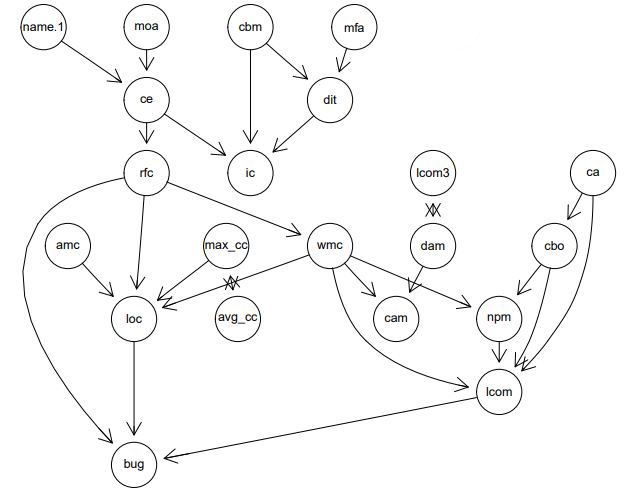
\includegraphics[width=8.5cm]{images/ANT_1.7_Graph.png}
% \end{figure}
%  generated by pcalg \(\alpha = .01\) from all the sample.



% Figures 1 and 2 showcase two causal graphs generated by the pc function of the pcalg package in R\cite{PCALG1} with the same parameters on datasets from two release versions 1.5 and 1.7 of the ant software.  These causal graphs were generated specifically using the "stable" \cite{colombo2013orderindependent}\cite{PCALG1} option of the pc function and yet they display large differences in the edges contained in the graph.  Not only are these edges unstable but they display direct contradictions.  One such contradiction is the connection and causal relationship from the node rfc which represents the response for a class and bug which is the total number of bugs; in version 1.5 there is a direct causal relationship from bug to rfc labeling bug as the cause and rfc as the effect, whereas in version 1.7 this relationship is actually reversed.  Another difference is that version 1.5 has lcom3 and dam independent to the rest of the graph whereas in version 1.7 these are not conditionally independent from the rest of the graph as they have a bearing on cam.  Note that not all variables are found in these graphs, this is because these variables were deemed conditionally independent from the other variables in the dataset, so they were omitted. 



\section{Experiments}\label{xp}

\subsection{Methods}
The last section made the case that causal graph instability in SE {\em might} matter since it could confuse a range of important tasks (analysis, reliability,
interventions, scalability, decision-making). But so far, this paper has only offered evidence of instability 
  from one data set (in Figure~\ref{cause1}).


The experiments of this paper make the case that instability in causal graphs is a widespread problem. To do that, we check for the prevalence of causal graph instability seen in Figure~\ref{cause1}. 

  % All experiments were run through the same experimental rig, modifying one variable and leaving everything else constant in order to isolate and evaluate various sources of instability individually.  The packages used in the implementation and execution of these experiments were dplyr\cite{dplyr} and pcalg\cite{PCALG1}\cite{PCALG2}



\subsubsection{Data sets}
We explored six defect data sets from widely used open-source JAVA projects.
These projects contain static attributes that describe thousands of classes (using the attributes listed in   Table~\ref{words}). The datasets used are from Jureczko et al.~\cite{defectDatasets} and are versioned as follows:
\begin{itemize}
    \item  Ant versions 1.3-1.7, 
    \item Camel versions 1.0, 1.2, 1.4, \& 1.6, 
    \item Ivy versions 1.1, 1.4, \& 2.0, 
    \item Prop releases 1 - 6, 
    \item Velocity versions 1.4 - 1.6, 
    \item Xerces versions 1.2 - 1.4. 
\end{itemize}
 This data was then converted into a matrix using R~\cite{RSoftware} and then used in  the experiments detailed below.
 
\begin{table}[!t]
\begin{center}
\begin{tabular}{|l|l|l|c|} % Adjust the 8cm as needed
\hline
\textbf{Project} & \textbf{Release} &\textbf{Size} & \textbf{Percentage defective}\\ \hline
Ant & 1.3 & 125 & 16 \\ \hline
Ant & 1.4 & 178 & 22\\ \hline
Ant & 1.5 & 293 & 11\\ \hline
Ant & 1.6 & 351 & 26\\ \hline
Ant & 1.7 & 745 & 22 \\ \hline
Camel & 1.0 & 339 & 4\\ \hline
Camel & 1.2 & 608 & 36\\ \hline
Camel & 1.4 & 872 & 17\\ \hline
Camel & 1.6 & 965 & 19\\ \hline
Ivy & 1.1 & 111 & 57\\ \hline
Ivy & 1.4 & 241 & 7\\ \hline
Ivy & 2.0 & 352 & 11\\ \hline
Prop & 1 & 18471 & 15\\ \hline
Prop & 2 & 23014 & 11\\ \hline
Prop & 3 & 10274 & 11\\ \hline
Prop & 4 & 8718 & 10\\ \hline
Prop & 5 & 8516 & 15\\ \hline
Prop & 6 & 660 & 10\\ \hline
Synapse & 1.0 & 157 & 10\\ \hline
Synapse & 1.1 & 222 & 27\\ \hline
Synapse & 1.2 & 256 & 34\\ \hline
Xerces & 1.2 & 440 & 16\\ \hline
Xerces & 1.3 & 453 & 15\\ \hline
Xerces & 1.4 & 588 & 74\\ \hline
\end{tabular}
\end{center}
\caption{Dataset information, see Table~\ref{words} for information about variables.}\label{datasets} 
\end{table}
   

   
    

\subsubsection{Evaluation Criteria: the Jaccard index}
All our experiments compare pairs of causal graphs generated from our data.
 Given nodes $N$ for the independent variable (plus one for the class ``bugs"),  then a causal graph contains edges $E(N_1,N_2)$ that connect one node to another. For the delta between two graphs $G_1,G_2$
 with edges $E_1,E_2$ (that use the same nodes), we report the  
     number of shared edges, divided by the total number of edges:
     
    \begin{equation}
    J=\frac{|E_1 \cap E_2|}{|E_1 \cup E_2|}
     \end{equation} 

     This Jaccard index has the range $0 \le J \le 1$ where zero denotes no overlap and one denotes perfect overlap. We say that {\em larger} $J$ values indicate {\em more} stability.


\subsubsection{Experimental rig}
  All tests were run on a laptop with an AMD Ryzen 9 5900HX, 32 GB of RAM, and an Nvidia RTX 3070 laptop GPU. The graphs were generated by interfacing with the pcalg package for R, which can be located on the CRAN website~\cite{PCALG1} (and pcalg implements the PC algorithm discussed above).  
  The release version of the package is pcalg version 2.7-9, and the specific function experimented on is the PC() function located in the pcalg package \cite{PCALG1}\cite{PCALG2}.


 
\subsection{Results}


\subsubsection{RQ1: Do the projects demonstrate intra-project stability across releases?}

As shown in Algorithm~\ref{alg1}, this experiment compares the graph from one project
between  release $i$ and release $i + 1$.   
 To implement this, we iterated over our datasets for each of our six projects, generating a new causal graph for each version.  In order to keep everything consistent, we ran the ``stable" version of the PC function, with a full sample of each dataset, using the off-the-shelf defaults for
 our causal generator.  
 
  This algorithm is deterministic and will yield the same results every time it is run in this fashion. 
  
  This algorithm uses a default of $\alpha=0.01$ for maximum probability of rejecting the null hypothesis. We use that value here since 
with the example code shown in the  the manual for this package,
$\alpha$ is always set  to 0.01. In 
{\bf RQ3}, we experiment
with other values for $\alpha$.

 

 

\begin{algorithm}[h!tbp]
\footnotesize
	\caption{RQ1: Version Experiment Algorithm \newline\textbf{input: } d  datasets, used to generate and compare causal graphs.\newline \textbf{output: } a similarity report.}\label{alg1}
	\begin{algorithmic}[1]
		\For {($s \in \mathit{datasets}$)}
            \State $l \leftarrow newList()$
			\For {($v \in \mathit{s}$)}
				\State $m \leftarrow correlationMatrix(v)$
                \State $n \leftarrow numberOfRows(m)$
                \State $g \leftarrow pc(m, n, \alpha = .01)$
                \State $l.add(g)$
			\EndFor
            \State $exportAndSave(l)$
		\EndFor
    \State \textbf{Return} $compareSimilarity()$
	\end{algorithmic} 
\end{algorithm}

 

\begin{figure}[!b]
\caption{{\bf RQ1 results:} Graph of Jaccard Values across release, comparing release i to i + 1}\label{Version Instability}
\begin{center}
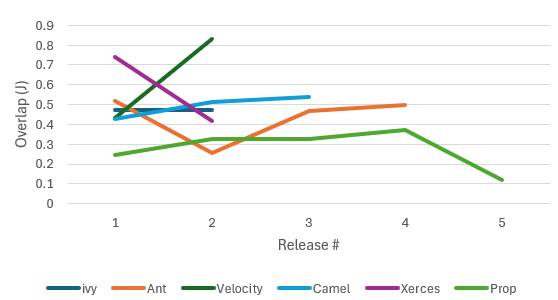
\includegraphics[width=8.5cm]{images/RQ1.png}\end{center}\label{rq1}
\end{figure}

Figure~\ref{rq1} shows the results. A slope between release $i$ and $i+1$ indicates that edges have changed between releases. Low y-axis values indicate poor overlap.

We note, in Figure~\ref{rq1}, that in nearly all our observations, the Jaccard index seems on the y-axis to be under 0.5; i.e., over half the causal connections found in one release are not seen in the next.
Hence, our answer to {\bf RQ1} is {\em that within one project across releases, there is much instability, despite running the supposedly ``stable'' version of the PC algorithm.  }



\subsubsection{RQ2: Do the graphs demonstrate inter-project stability across different projects?}
To answer this question, the goal of Algorithm~2 is to check if causal patterns hold in multiple projects. 
In order to observe this behavior we made the decision to use only the most recent datasets for all comparisons within this experiment.   The Prop dataset was excluded from this experiment as it contains differing variable counts which may impact graph generation beyond the intended scope of this experiment.



This experiment is deterministic and will yield the same results every time it is run in this fashion.
\begin{algorithm}[!h]
\footnotesize
    \caption{RQ2: Inter-Project Stability Experiment Algorithm \newline\textbf{input: }datasets,  being compared in this experiment\newline\textbf{output: }The similarity report for the causal graphs, exported and saved}
    \begin{algorithmic}[1]
        \State $graphList \leftarrow new List()$
        \For{(   $d  \in \mathit{datasets}$)}
            \State $m \leftarrow correlationMatrix(d)$
            \State $n \leftarrow numberOfRows(m)$
            \State $g \leftarrow pc(m, n, \alpha = .01)$
            \State $graphList.add(g)$
        \EndFor
        \For{($g \in \mathit{graphList}$)}
            \State $l \leftarrow newList()$
            \For{($i \in \mathit{graphList}$)}
                \If {$not g.equals(i)$}
                    \State $c \leftarrow compareGraphs(g, i)$
                    \State $l.add(c)$
                \EndIf
                
            \EndFor
            \State $exportAndSave(l)$
        \EndFor
    \end{algorithmic}
\end{algorithm}


\begin{table}[!b]
\caption{{\bf RQ2 results:} Inter-Project Jaccard Values. This matrix is symmetrical across the diagonal (so the values of blank cell $i,j$ can be found in
cell $j,i$).}
\label{tab:inter-project}
\begin{center}
\begin{tabular}{|l|l|l|l|l|l|} % Adjust the 8cm as needed
\hline
\footnotesize
\textbf{Project} & \textbf{Ivy} & \textbf{Ant} & \textbf{Velocity} & \textbf{Camel} & \textbf{Xerces}  \\ \hline %%\textbf{Prop} \\ \hline
\textbf{Ivy} & 1 & .28 & .37 & .25 & .26 \\ \hline%%& 0 \\ \hline%%\\ \hline
\textbf{Ant} &   & 1 & .28 & .19 & .20 \\ \hline%%& 0 \\ \hline%%\\ \hline
\textbf{Velocity} &   &  & 1 & .20 & .26 \\ \hline%%& 0 \\ \hline
\textbf{Camel} &   &   &   & 1 & .29 \\ \hline%%& 0 \\ \hline
\textbf{Xerces} &   &   &  &   & 1 \\ \hline%%& .02 \\ \hline
%%\textbf{Prop} &   &   &   &   &  \\ \hline%%& 1 \\ \hline

\end{tabular}
\end{center}
\end{table}

Figure~\ref{tab:inter-project} shows the {\bf RQ2} results.
The Jaccard values indicate that around 75\% of the causal connections
found in one project are not present in the other
(exception: for  Ivy and Velocity, that overlap is 40\%). 
Hence, our answer to RQ2 is {\em that there exist wide, large  
 inter-project instabilities indicating very little consistency between graphs generated by the PC function on data from different projects.} 

To say that another way, at least in the corpus studied here, it would
be misleading to use causal graphs to report supposedly general causal effects with the JAVA open-source projects
studies in this analysis.





\subsubsection{RQ3: Does parameter tuning affect stability?}
The third research question is concerned with tuning parameters in order to display potential additional sources of instability in the generator.

All learners come with ``magic'' tuning parameters that can
change and improve a learner's performance. Different data
sets can benefit from different tunings~\cite{fu2016tuning}. 

For example, the causality package used here is a tuning
parameter controlling the significance level or \(0 \le \alpha \le 1\), that sets a threshold for the conditional independence tests used in the PC function.  The lower the significance level, the lower the chance of a Type I (or false-positive) occurring, and the higher it is, the higher the chance of a Type II error. This significance level also has a bearing on the total edge count of the graphs produced by the function, and the closer it gets to 1, the more edges the graph has.  Additionally, the smaller it gets, the number of edges in the graph appears to decrease all the way to very little or no edges.  

The default value for $\alpha$ in  our package is
$\alpha=0,1$, but researchers are free to change that value. For each data set, as shown in Algorithm~3,  we generated graphs from the latest version of the system, using  999 different 
$\alpha$ values ranging from  .001 to .999.  These graphs were compared to those found using $\alpha=0$.


\begin{algorithm}[h!tbp]
\footnotesize
    \caption{RQ3: Parameter tuning   with significance level (\(\alpha\))\newline\textbf{inputs: }datasets,  used to generate the causal graph d\newline\textbf{outputs: } Similarity report, exported and saved}
        
    \begin{algorithmic}[1]
        \For{($d \in \mathit{datasets}$)}
            \State $graphList \leftarrow  newList()$
            \State $m \leftarrow correlationMatrix(d)$
            \State $n \leftarrow numberOfRows(m)$
            \For{$i \in {0...998}$}
                \State $sigLev \leftarrow (.001 + (i /1000))$
                \State $g \leftarrow pc(m, n, \alpha = sigLev)$
                \State $graphList.add(g)$
            \EndFor
            \State $g1 \leftarrow graphList.get(0)$ 
            \State $l \leftarrow newList()$
            \For{($i \in {1...998}$)}
                \State $g2 \leftarrow graphList.get(i)$
                \State $c \leftarrow compareGraphs(g1, g2)$
                \State $l.add(c)$
            \EndFor
            \State $exportAndSave(l)$
        \EndFor
    \end{algorithmic}
\end{algorithm}

Before reviewing the results, we state our pre-experimental expectations. Our prior work on hyperparameter optimization showed that tuning can have small to medium effects on the veracity of the output (e.g., 10 to 30\% improvements in recall). These effects are often linear on the magnitude of the tuning~\cite{fu2016tuning}. Hence, our
pre-experimental expectation was that changes to $\alpha$ would produce some, but perhaps not large, gradual changes to the causal
graph.



\begin{figure}[!t]
\caption{{\bf RQ3 results:} Graph of Jaccard values when shifting alpha \(\Delta = .001\). All graphs comapred to the graph from $\alpha=.001$.}\label{Variable tuning graph}
\begin{center}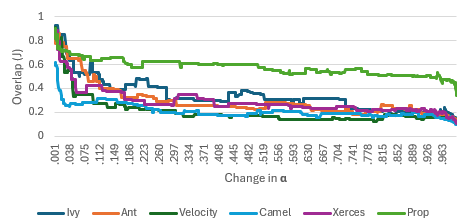
\includegraphics[width=8.5cm]{images/RQ3.png}
\end{center}
\end{figure}

The {\bf RQ3} results are shown in results. 
At larger $\alpha$ values (e.g. $\alpha > 0.2$), we can see the gradual and small changes suggested by our pre-experimental intuitions.
However, at lower $\alpha$ values (e.g. $\alpha < 0.1$), very small changes
in this parameter can lead to very large changes in the graphs (e.g., consider the range $0.025-0.075$ where many of data sets exhibit precipitousness drops).
 
The concern here is that brittleness in the resulting graphs is not documented
in the support material for this package. Hence, users of this tools might make a seemingly innocuous (and very small) change to $\alpha$ without realizing that that change can have a dramatic impact on the generated graph/


% are shown in 
% As visible in the figure above one can observe how even small shifts in significance level when testing for conditional independence yield vastly different graphs.  As the \(\Delta\alpha\) increases the Jaccard values decrease, however, one important note is that the shift is most prominent within the first one to two hundred graphs (alpha shifting from .001 to approximately .2 with an individual \(\Delta\) of .001).  This is important because the most commonly used values for alpha in statistics are .01 and .05 which fall within this range of significant instability, even at a small delta. However, if a test without a lot of power is needed, where false negatives are of higher concern than false positives one may use higher values for the significance level and begin approaching a value of one depending on how important it is to avoid false negatives for that individual use case.  As such this comprehensive test displays how just tuning this one variable leads to a wide source of instability that is fairly consistent across datasets. 

Aside:  One additional thing to note about this result is how the Prop dataset is less impacted by the significance level, we are unsure why this is due to the limitations of available datasets.  Our current hypothesis is that this may have to do with the size, as all of the other datasets are of similar sizes, and exhibit similar end behaviors, while the prop is nearly one hundred times larger, making this seem like the most likely source of such a prominent disparity between the sets. 
 That said Prop still exhibits the same behavior, just to a less extreme extent as alpha decreases.  Other parameters could be modified and potentially may be sources of further instability, but just modifying the significance level displays a potential instability source.  


Overall, our answer to {\bf RQ3} is {\em that tuning the parameters, specifically the significance level or \(\alpha\) can lead to significant instability in the graphs output by the generator.}

 
\subsubsection{RQ4: How much do causal graphs change if we remove only small fractions
     of the training data?}
The final research question explores what happens if we make a small
change to the training data used from graph generation. 
Here, we defined ``small'' to be ``remove 10\% of the data, selected at random''.
For each data set:
\begin{itemize}
\item This experiment ran for 20 times 90\% sub-samples of the data.
\item 19 of the graphs were compared to the first graph generated.
\end{itemize}
Before reviewing the results, we state our pre-experimental expectations: 
we expected that   removing  merely 10\% of the data should not have a large impact
on the generated edges.

 
\begin{algorithm}[h!tbp]
\footnotesize
    \caption{RQ4: Intro-Project 90\% Subsampling Algorithm\newline\textbf{inputs: }datasets  used to generate the causal graph d\newline\textbf{outputs: } Similarity report, exported and saved}
    \begin{algorithmic}[1]
         \For{($d \in \mathit{datasets}$)}
            \State $graphList \leftarrow newList()$
            \State $sampSize \leftarrow ceil(.9 * d.getRows())$
            \For{$i \in {0...19}$}
                \State $sample \leftarrow sample(d, sampSize)$
                \State $m \leftarrow correlationMatrix(sample)$
                \State $g \leftarrow pc(m, sampSize, \alpha = .01)$
                \State $graphList.add(g)$
            \EndFor
            \State $g1 \leftarrow graphList.get(0)$ 
            \State $l \leftarrow newList()$
            \For{($i \in {1...19}$)}
                \State $g2 \leftarrow graphList.get(i)$
                \State $c \leftarrow compareGraphs(g1, g2)$
                \State $l.add(c)$
            \EndFor
            \State $exportAndSave(l)$
         \EndFor
    \end{algorithmic}
\end{algorithm}

\begin{figure}[h]
\caption{{\bf RQ4 results:} Graph of 90\% subsample Jaccard values from datasets}\label{Subsample graphs}
\begin{center}
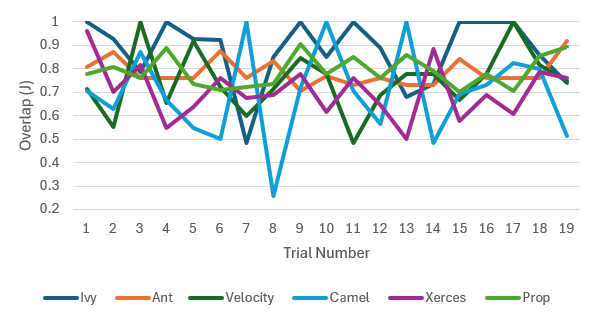
\includegraphics[width=8.5cm]{images/RQ4.png}
\end{center}
\end{figure}

The results did not meet our expectations.
As seen in Figure~\ref{Subsample graphs}, the Jaccard index between graphs vary wildly between Jaccard's of .6 to 1 with some observations slipping as low as .25.  As these sub-samples were generated randomly there is a risk of obtaining certain outliers in the dataset resulting in significantly different graphs, so more trials would be necessary to determine which datasets in particular are more susceptible to this behavior.  That said,   .6 to 1 is still a fairly wide zone of variability.     

Overall, our answer to {\bf RQ4} is {\em that instability is not always present in a 90\% subsample, at least relatively compared to the other experiments.  In the subsample experiments, most of the Jaccard values were in between the range of .6 to 1, and while this still represents a fair amount of variability across all of the datasets this is nothing as low as the yields from the other experiments.}

\section{Discussion}\label{discuss}
\subsection{Threats to Validity}


\textbf{Internal validity}  is the degree of confidence that the causal relationship you are testing is not influenced by other factors or variables.
We have tried a range of factors that might cause instability (intra-vs-inter project changes, a hyper-parameter change, some sub-sampling) and large instability was seen in all cases. 
 
\textbf{Sampling bias  } refers to instabilities in the conclusion due to
the data used in the study. No data mining study can explore all data sets
and it is possible that the instabilities seen here are some quirk of defect prediction data. In terms of future work, it would be useful to determine if different kinds of data generate more/less stable causal graphs.

\textbf{Construct validity} 
 is about how well a test measures the concept it was designed to evaluate.
 Our measure of instability is the Jaccard index, which looks at the internal edges of a graph. An alternate measure might be to ignore the internals and just ask what inputs usually lead to what outputs. That said, we know of no publication using that measure.

\textbf{Dependability:} 
Non-deterministic experiments introduce a threat to validity (since   conclusions may   be a quirk of the random number generator). Most of our experiments are deterministic, with the exception of {\bf RQ4}.
To mitigate this threat to validity, we ran {\bf RQ4} 20 times with different random number seeds.

 
\subsection{Future Work}

We hope this paper inspires much subsequent research. For example:
\begin{itemize}
 
    % \textbf{What attributes of a dataset promote or reduce stability? Can we c}  If these techniques can be used to promote stability which ones work best and do they work consistently across a variety of datasets? Additionally, do any techniques actually reduce the stability and should be avoided if the intention is to perform causal inference on the generated data using a graph generator?  Are all generators and algorithms impacted similarly by these techniques if there is an impact, for example, do data pre-preocessors like
    % SMOTE~\cite{chawla2002smote} impact stability?  If attributes such as size and minority classes promote instability, how can these be resolved in a way that yields valid, logical, and consistent results that are still useful and actionable?
 \item   

 \textbf{How to mitigate for instability?} Do stochastic approaches improve stability? Does lowering the significance level when testing for conditional independence promote stability as it decreases false positives and reduces the overall total edge count? If the decreasing significance level does promote stability what is a desirable significance level to choose so the graph can still be useful while also being consistent? Additionally, can the correct tuning parameters be automatically selected  in order to tune them properly for a given dataset to make the best guess at what the correct configuration would be if one exists to generate reliable causal graphs for that dataset?

 
% \textbf{What additional generators exist, and how do they fair in terms of stability relative to pcalg?} Additionally, how do the other algorithms of causal inference compare to the results of this study?  
% Additionally, what other algorithms are most commonly employed for causal inference beyond the Peter-Clark algorithm as a baseline.
% If other algorithms exist as common baselines for pieces of software what are they, how do they work, and how do their results validate or contradict the results of this study on the stability of causal inference?

\item
    
    \textbf{What is the impact of instability on the use cases of causal graphs?} How could the instability detected in this study impact different ways people use causal graphs? For example, when diagnosing faults, is causal graph instability actually a good thing (since it generated more options)? Or, can the same final answers be obtained through different means across different graphs?   
    
% \textbf{What other potential applications are there for these graphs?} Do they have broader applications within the software engineering field?  If so are there particular datasets that these graphs perform better with, this study indicated that this may be the case as during the parameter tuning experiment the Prop dataset fared significantly better than the rest of the datasets in terms of stability.


   \item 

    \textbf{Beyond the Jaccard index, are there better ways to evaluate the structure of a causal graph?}  If so, how can this value be optimized, and is this a metric that can be consistently applied and evaluated in graphs automatically?  Additionally, would it be possible to use an evaluation function for a graph generator to promote stability? For example, if a causal relationship is known before running the generator, can this evaluation function be asserted so the generator begins with a partial graph? And would this promote stability and/or utility between graphs?  
    
% \textbf{How important is stability in the study, and are the results presented by a causal graph still useful if they are not consistent?} If the graphs themselves are not consistent is it reasonable to assume that the observations generated from them really mean or imply anything at all? If this assumption is made should it be verified by several graphs? For example, even in the experiments that resulted in less consistent results with lower Jaccards, there were still certain edges that appeared in almost every graph, are these edges more valuable because they are more consistent, or do they display a higher level of confidence in the existence of that relationship?

 % \textbf{For the current applications of causal graphs, if instability poses a large risk what are potential alternative solutions?} If the risk of instability in generated graphs is a large risk then how can this be worked around? Will several graphs need to be generated and compared in order to find one that best suits the problem, and how could this be determined in a reasonable time period without just using every graph until you find one that indicates correct relations?  Additionally, is it possible to generate a causal graph that directly leads to the source or cause of an issue in a complex environment both accurately and consistently given enough complete data?
 
\end{itemize} 
\section{Conclusion}
Our reading the literature is that causality is a topic of growing interest in software engineering. But something can be widely used and still be wildly misleading.
The experiments of this paper have
demonstrated  causal graph instability:  
\begin{itemize}
\item Across different releases of the same project (see {\bf RQ1});
\item Across different projects (see {\bf RQ2});
\item Across tuning changes to the data of one project (see {\bf RQ3});
\item And even across very small changes (10\%) of the training data (see {\bf RQ4}).
\end{itemize}
From these experiments, and our literature review, we make four observations:
\begin{enumerate}
    \item
Many SE researchers do not appreciate the frequency and impact of causal instability.
\item
Before using causal graphs  to make   general claims about software development,  SE researchers need to test   that any such conclusion 
 {\em holds over the numerous causal graphs} that we might generate from the same data.
 \item
Unless the second point is satisfied,  we should not use causal graphs as a way to generate the models
that are reported to business users or the research community.
\item 
As recommended by some statisticians, perhaps it is best to use causal graphs as a verification tool.  
 Sibert~\cite{SIEBERT2023107198} argues that 
{\em 
``The main purpose of such a (causal) graph is to reason about the presence of potential spurious correlations
that may bias the analysis''}.
In this view, causal graphs are an interim, possibly throw-away, model that is generated and inspected before moving on, perhaps to some other modeling methods
\end{enumerate} 
As an example of the last point,  based on our background knowledge of software engineering, we suspect that there is something very wrong about 
 the data used to create Figure~\ref{cause1}.a.  Lines of code should  {\em cause} bugs (and not the other way around).  Hence, before doing anything else with the Figure~\ref{cause1}.a data, there needs to be some investigation into that anomaly.

 
% Overall our experiments yielded large examples of potential instability in graphs generated by the PC algorothm for use in software engineering, across versions, between projects, when tuning parameters, and to a lesser extent when taking a random subsample of the same dataset.  These sources of instability can be drastic and actually result in ancestor nodes becoming children, or independent nodes becoming entirely dependent.  This is concerning, because if the desire is to utilize this software for complex tasks such as root cause analysis, how could this task be accomplished with any amount of consistency if the graphs generated suffer from wide instability?  Our results indicate that there is large-scale instability expressed by the implementation of the PC algorithm in the pcalg package when tested against software engineering datasets.  This is concerning regarding our experiments because if one of the accessible baseline approaches has inconsistencies and sources of instability, has this issue propagated forward to any generators produced using the PC algorithm or taking inspiration from an available implementation of it?  There are also currently large difficulties in the field of software engineering for evaluating and working with causal reasoning in research.  This is caused by a lack of resource availability, clarity on the new techniques, and a lack of consistency in ways to draw conclusions from the research currently done due to the novelty of the approaches and gaps present in the current research which may continue to impede future endeavors for some time.
% \subsection{RQ1}
% Our experiment associated with RQ1 yielded results that presented a wide source of instability between releases of a singular project from release i to i + 1.  This is particularly worrying due to the common nature of comparing software data across releases.  This may represent a potential issue in the application of software that is reliant on such causal inference algorithms.  An additional area of concern is the varied results and the lack of consistency even among the instability present between the releases.  Some observations represent a relatively stable graph such as between the two most recent releases if Ivy examined, while others did not fair as well such as Prop from release to release.  It is possible that there is some attribute or characteristic of the datasets that promotes or hinders cross-release intro-project stability, but this is something that will need to be examined in future work.  
% \subsection{RQ2}
% Our experiment associated with RQ2 yielded results of significantly large instability, showcasing that there is very little stability in the graphs generated between the most recent release dataset of various projects.  Since it is reasonable to make observations about data from one piece of software and apply it to another project this instability is not expected, to this extent, nor is it desirable.  This may also indicate a potential issue in the use of such generators to perform root cause analysis, or to aid in performing root cause analysis beyond initializing discussion.
% \subsection{RQ3}
% Our results from RQ4 indicate that altering the significance level does have bearing on the stability of causal graphs generated.  This difference is much more prominent for the first couple increases as the curve levels out as the significance level gets farther away from where it starts.  Most studies will not use significance levels which are in the part of the curve that is leveled out, between the values of .01 and .05, for \(\alpha\) (both of which are relatively common values) the curve of stability when measured by the Jaccard coefficient decreases very quickly even with a \(\Delta\) as small as .001.  
% \subsection{RQ4}
% Our results for RQ4 indicate that 90\% subsamples of the data can be sources of some degree of instability with the Jaccard values between any two graphs mostly being between 1.0 and 0.6.  This was definitely the most positive result of the four experiments in favor of the stability however though, as these graphs appear to be relatively stable compared to the ones yielded by the other experiments with some differences from graph to graph being caused by the omission of a random 10\% of the dataset.


%% Detail potential remaining unanswered questions and remaining areas of interest that could be picked up by a later study, think additional parameters, other generators, more datasets, CI tests, etc.

%% Gather all sources used throughout the semester and specifically the ones used in this paper (mainly in lit review section and format them appropriately here

 

% \section{Literature Review}

% \subsection{Existing Software and Applications}


% The software engineering literature about causal graphs presents a wide array of potential implementations, software, and algorithms to produce causal graphs. 
% All of these graphs are directed graphs that attempt to represent a causal relationship between two variables.  Some pieces of software that generate causal graphs to perform their task(s) include microScope, Groot, PerfCE, CauseInfer, Sieve, and Sage.\cite{MicroScope}\cite{Groot}\cite{PerfCE}\cite{CauseInfer}\cite{SIEVE}\cite{sage} The most common through line in the application of these pieces of software is to be used as a tool primarily for root cause analysis and/or fault localization.  The point of root cause analysis is to try and determine the overall cause of a given state, outcome, or event, the nature of these questions and causality make causal graphs seem like a good structure to perform this task.  Another main source of interest in causal graphs for this cause is due to the decrease of monolithic architecture in software in favor of using complex software that is reliant on multiple interdependent microservices.  The microservice architecture has many positive benefits including the aid in scalability and efficiency of software development.\cite{MICROSERVICE} However, they do serve to increase the complexity of tasks such as root cause analysis as multiple services become interdependent to perform complex operations.   Sieve, Sage, and microScope\cite{SIEVE}\cite{sage}\cite{MicroScope} are three technologies aimed at mitigating some of the complications in software processes that can arise with the increase in system distribution. 
% Additionally, there are even larger, broader potential applications for this technology even potentially extending beyond the field of software engineering.  Some of these applications include biology\cite{PCParalell} outside of software engineering, and metamorphic testing within software engineering\cite{METAMORPHIC}. These represent a subset of the areas of interest for the potential application of this technology.  It is stated in the literature in ~\cite{SIEBERT2023107198} that the purpose of a causal graph is:

% \begin{quote}
%     {\em The main purpose of such a graph is to reason about the presence of potential spurious correlations that may bias the analysis}
% \end{quote}  

% In this quote it is asserted that the primary purpose of such causal graph data structures is to reason about the presence of anomalous or incorrect relationships.  We have concerns with this application being the intended purpose, as instability may cause the causal graphs themselves to also be spurious under the proper conditions.
% It is also noted that this field of research is very fragmented with a lack of consistent, agreed-upon evaluation or implementation techniques which serves as a current roadblock for the current furthering of research.\cite{SIEBERT2023107198}.  To back this claim, in \cite{Groot} it is mentioned that all other causal tools for root cause analysis reviewed in their literature, including CauesInfer\cite{CauseInfer} and MicroScope\cite{MicroScope} have either not been validated on real incidents based on their review or had only partially been validated.  This is an important gap in the experimentation done to present in the available research on causal reasoning and one that is important for understanding the applications of such systems. Additionally in the literature presenting Groot \cite{Groot} they mention how there are motivating results of their causal system for root cause analysis as an event-based graph generator in order to draw observations about a dataset and the relationships between variables.  This leads to the idea that they claim that they have utilized causal reasoning in order to successfully and reliably perform root cause analysis.  
% This is expressed when in ~\cite{Groot} when they evaluate their results and say:

% \begin{quote}
%     {\em The top-1 and top-3 accuracy is calculated as the
%  percentage of cases where their ground-truth root cause is
%  ranked within top 1 and top 3, respectively, in GROOT’s results.
%  GROOT achieves high accuracy on both incident categories.
%  For example, for business domain incidents, GROOT achieves
%  96\% top-3 accuracy.}
% \end{quote}

% This is relevant because it shows the claim that GROOT identifies the Root Cause Analysis within the top 3 96\% of the time in a real-world application utilizing causal graphs ( 81\% for the top 1 case).  They go on to take it one step further, asserting that the remaining failing cases are caused by missing/omitted events in their graph generation.  The results of this experiment appear extremely promising for the use of causal inference and graph generation in the field of software engineering, at least for root cause analysis.  Additionally, GROOT has a UI component which is intended for SRE teams to draw conclusions from the visual graph representations, this is presented from ~\cite{Groot} with the quote:

% \begin{quote}
%     {\em GROOT currently supports daily SRE work...Note that all causal links in the UI indicate "is cause of" being the opposite of "is caused by"... to provide for a more intuitive UI for users to navigate through. GROOT visualizes the dependency and event causality graph with extra information such as an error message.  The SRE teams can quickly comprehend the incident context and derived root cause to investigate GROOT further.}
% \end{quote}

% In this quote it is stated that clients, in this case SRE can easily make observations about the root cause based on the analysis performed by GROOT and the graph generated.  This combined with the previously stated consistency and accuracy, make it that the outlook on this technology certainly does seem very positive.  Even more so because there is a later section in the GROOT \cite{Groot} paper where they detail SRE feedback to the technology which seems to be very positive, implying that GROOT is effective, accurate, and user-friendly.
% However, here and in most other pieces of literature reviewed for this study there is no publicly available implementation of this software, and stability is not explicitly checked in this paper.  If stability is not checked there is a severe potential that graphs being relied upon for root cause analysis may yield incorrect results, and potentially waste time or result in an incorrect diagnosis. In spite of this potential limitation, however, results are still being shared and seem to have a positive outlook, at least based on what is provided in the literature in their results.  
% As demonstrated in .~\cite{DATASHIFT} where they generate a causal graph and utilize it for a fault localization experiment:

% \begin{quote}
%  {\em SimpleClaimsStream is identified as the most likely source of the observed shift, and as this stream is an output of the ClassifyClaimComplexity node, we can correctly deduce that this node is indeed the source of a problem.}
%  \end{quote}
 
% In this experiment, they purposefully inserted a bug into the portion of the code represented by the \(SimpleClaimStream\) node.  Their research shows that using their causal inference algorithm they are able to view this output and say that the most likely source of the fault is at that node, which in this case is correct.  This demonstrates a potential application of this technology in action, but also an area of concern, as this was on a seemingly relatively small-scope experiment.  We worry that issues with stability may not present themselves as clearly in smaller experiments with fewer variables, resulting in the claimed consistency of this result.  This consistency is presented when they say ~\cite{DATASHIFT}

% \begin{quote}
%     {\em Welch's t-test gives \(p < .001\) indicating statistical robustness of our procedure in identifying the source of the bug in this experiment.}
% \end{quote}

% After running this experiment they rerun it 30 times with randomized data presenting an encouraging result of this particular software application with less than a one percent chance of being incorrect.  Once again, however, this paper does not expressly examine or account for the stability of the individual graphs generated, and whether any instability present will have a negative impact as this technology is scaled up to work in more complex environments outside of the experimental space.

% In \cite{BIASINRESULTS} it is mentioned that in their literature review, they were unable to fully and fairly answer the question of whether or not causal inference was useful in these software applications due to how little information was made available.  This seems to be a common struggle throughout the field right now, which as a whole appears both new and fragmented in its current state.  

% \subsection{Underlying Algorithms and Implementation}
% One source of difficulty in analyzing software used in relation to causal graphs that is noted in some literature is that most code is not made available.  This makes it extremely difficult to evaluate the efficacy of these tools, this problem has been documented in other studies too. \cite{SIEBERT2023107198} Additionally, some papers do not share implementation for reproduction nor do they explicitly share results which makes information incredibly difficult to verify, contradict, or agree with.  However, some of the literature, and its associated software do make their algorithms known more publically, or at least the basis of those algorithms.  Specifically, CauseInfer\cite{CauseInfer}, and MicroScope\cite{MicroScope} both utilize implementations of the PC algorithm\cite{kalisch2007estimating} to generate their causal graphs.  This algorithm is a baseline algorithm of causal inference which historically has had a variable ordering problem\cite{PCParalell}.  This has been mitigated by a later "stable" PC algorithm through modifications\cite{PCALG1}\cite{colombo2013orderindependent}.  The reason for the widespread use of this algorithm as a baseline, underlying inspiration, or component of an implementation is multifaceted.  Two large reasons are that the PC algorithm is feasible for computation on a larger scale with several variables.  It is also known to be consistent in graphs containing several variables, or dimensions \cite{colombo2013orderindependent}.  One additional bonus is that there are open-source software projects that contain available use of this code, giving it to the public and anyone looking to make their own software reliant on causal reasoning.  This becomes especially important when remembering the lack of available implementation of other, newer generators and their algorithms\cite{SIEBERT2023107198}, this pushes people towards these open-source resources that are available to use as baselines when creating their own generators, or software reliant on causal inference.  As such the weight of such packages becomes more important.

% \subsection{The pcalg package}
% One such package referenced in the literature is called pcalg \cite{PCALG1}
% \cite{colombo2013orderindependent}\cite{PCParalell}.  This is a package in R that is located and can be downloaded from the CRAN network which is an official archive of verified package releases to be used in R.  The pcalg package is the package listed to utilize for causal inference in R.  This package has multiple methods of generating causal graphs which are implementations of various algorithms, including, FCI, GFCI, and PC. However, the one we will focus on in this paper is the pc() function which is this package's implementation of the PC or Peter-Clark algorithm.  The reason we choose this package, and this algorithm is the limitation of available implementations of newer generators, and that of all of the SE literature reviewed during this research we found that the PC algorithm was the most commonly used baseline algorithm presented.  The others present in the package were occasionally mentioned but were not explicitly provided as a used underlying algorithm in software.  The three main applications of the PC algorithm, either as a baseline or as an internal and essential component of the graph generation were CauseInfer\cite{CauseInfer}, MicroScope\cite{MicroScope}, \& the parallelized PC algorithm implementation that was developed to try and improve the speed of the algorithm consistently across the board\cite{PCParalell}.  In the particular case of the literature regarding the parallelized PC algorithm, it is specified that they utilized the implementation of the PC algorithm in the pcalg package in order to generate their version of the algorithm which parallelizes various components of the algorithm, which had proven to be a challenging task for some time, as the algorithm is sequential in its steps.  After its initial release, the pcalg package received an update adding a stable variant of the algorithm aimed at fixing the variable ordering issue present in the package\cite{PCALG1}.  This is the variant of the algorithm we will utilize in this project to promote stability as much as possible when performing our experiments.

\newpage \section*{Conflict of Interest Statement}

The authors declared that they have no conflict of interest.


\section*{Data Availability Statement}

The authors declare that the data and scripts supporting the findings of this study are available  at
\url{https://github.com/jphulse/Stability_Of_Causal_Graphs_Public}.

% Beginning of formal reviewer feedback for revision
\newpage
\pagenumbering{roman}
\setcounter{page}{1}

\section*{Response to Reviewers}

The reviewers agree that your paper targets an interesting set of questions, which have received insufficient attention in previous work. They also agree that the paper is generally clearly written and easy to read.

At the same time, all reviewers also pointed out a few important shortcoming in how the paper's research, and found that the paper currently lacks enough substance and depth to be acceptable for publication in EMSE.

\BLUE{Yes, we completelyagree. The previous version only studied one causal graph generator  (PC) for one SE tasks (defect prediction). This revised paper now studies multiple causal graph generators (including new ones,  recommended by the reviewers) and multiple SE tasks. As shown in our new results, these new experiments confirm
our old conclusions. That is, just like LLMs, all the causal graph generators we study here suffer from hallucinate and, for a wide range of tasks,  can offer misleading conclusions. } 

Overall, I recommend that you undertake a major review, focusing in particular on the following key points of criticism:

1. (R1, R2) Discuss the assumption that the causal discovery algorithms rely on, and whether they are applicable to the scenarios where they are normally applied. This is important both to frame the research presented in the paper, as well as to ensure that the empirical comparisons are consistent and fair.

\there{e1}{Yes, this is a good point. This section now has a extensive discussion on how the causal framing of this work. f}

\BLUE{We agree. The previous version only studied one causal graph generator  (PC) for one SE tasks (defect prediction). This revised paper now studies multiple causal graph generators (including new ones,  recommended by the reviewers) and multiple SE tasks. As shown in our new results, these new experiments confirm
our old conclusions. That is, just like LLMs, all the causal graph generators we study here suffer from hallucinate and, for a wide range of tasks,  can offer misleading conclusions. } 

2. (R1, R3) Consider using additional datasets from different domains, or at least include additional variables (such as function-level metrics), which is necessary to improve validity. This could help address the criticism that: (R1) the variables available in the datasets used in the paper are likely missing key information that would be necessary to extract meaningful causal relations; (R3) the defect domain is not the main domain where causal graphs are used, and thus the findings may not generalize.

3. (R1) Since this is crucial background information for the paper's main contributions, extend the discussion of existing causal discovery algorithm (following some of the suggestions given by the reviewers).

4. (R3) Related to the previous point, and most important, consider additional causal discovery algorithms in your experiments.

5. (R2) Discuss the "ground truth" accuracy of causal discovery algorithms, also in relation to non-algorithmic causal modeling (i.e., done by domain experts). This can also help better frame the paper's contributions, and any consequences thereof.

Thoroughly addressing these points is necessary to add enough critical mass to the paper, so that it can be considered for a journal-first publication in EMSE. In addition, please make sure to respond to all (other) points mentioned in the reviews, and explicitly point out which parts of the paper you changed or added to address each point.

Please complete your revision and submit it together with a list of changes and rejoinder to the reviews.




% Please add the following required packages to your document preamble:
% \usepackage[table,xcdraw]{xcolor}
% Beamer presentation requires \usepackage{colortbl} instead of \usepackage[table,xcdraw]{xcolor}

\begin{enumerate}
    \item Response to Reviewer 1
    \begin{enumerate}
        \item The paper should discuss in more depth what causal discovery (also called causal structure learning) is and what are the assumptions behind causal discovery algorithms are.
Especially:
- Sufficiency: the assumption that there is no unmeasured confounder.
- Linearity / non-linearity of the causal effects.

This is relevant since the PC algorithms does assume sufficiency and linear effects. There are other algorithms (like PCI) that relax these assumptions (see Vowels et. al Definitions and Table 1). \\{\MARK \dots}
    \item The experimental setup is a little bit light.
- The dataset used (by the way, you forgot to mention the source or I missed it in the manuscript, so I am assuming the data comes from the PROMISE or Unified Bug datasets) only contains code metrics + number of bugs. These variables and their relationship to #bugs is influences by factors that are difficult to measure (problem complexity, testing effort, developers skills), see for instance [Fenton and Neil, 1999]. Therefore the PC algorithm is, because of it assumes sufficiency, not really suitable for extracting a causal graph (at least not if we are interested in the relationship between code metrics and \#bugs).
- I know that you are using class level metrics, which makes hard to build a causal graph in the first place, but there might be some edges that we know are causal (like number of lines of codes does have an impact one the number of notes, maybe not direct, but there should be no arrow going from #bugs to loc). By using function level metrics, we were able to derive some partial causal graph that we could test upon. It would be interesting to see whether some causal edges can be derived from the definitions of the metrics, and whether these are found by the causal discovery algorithms.
- It is kind of obvious that changing hyperparameters such as alpha will change the number of edges found by the PC algorithm. However the fact that some edges are detected for longer ranges of alpha values is interesting. We also found a similar behavior, and hypothesized that this could be linked to the fact that some edges are more robust because they might be real causal edges (under the assumptions followed by the causal discovery algorithm). We did not investigate it much. In fact a proper treatment of this problem would require to investigate research in the field of hyperparameter tuning in causal discovery algorithm (see Machlanski et al, Biza et al.). \\{\MARK \dots}
\item Detailed feedback for section 2.1:
\begin{enumerate}
    \item You write: << Different levels of human cognitive styles, says Pearl, match different levels of this hierarchy. For example, merely reporting "what is?" via correlation (or some method that infers y = f(x)) is level one. Deciding "what to do?" (i.e. what interventions to take) is a higher-level task that is more cognitively difficult. This requires questions about "what if?" and "what if I do X?". Finally, above the "doing" level is the "imagining" level that explores issues of "why?" and "was it X that caused Y?" and "what if I had acted differently?" >>, it is not "different cognitive styles", Pearl showed that for each level you need different mathematical tools (level-1: correlation, level 2: do-calculus, level 3: counterfactual reasoning) and that you cannot use tools from level i to answer questions on the level i+1. \\{\MARK \dots}
    \item Your write: << In these graphs, when there is an edge between any two nodes, X and Y, going from X to Y, one can imply that X has a causal effect on Y. >>. You cannot imply that X has a causal effect on Y, you are assuming that this is the case. The causal graph is a model (a simplification of a given system, used to answer a certain question on that system), that represent the modelers assumptions. \\{\MARK \dots}
    \item I am not sure what you mean in the next sentence: << This is combined with asserting that given all other additional random variables in the set, there is no variable Z for which X and Y exhibit conditional independence [44] [24], within a threshold. >>. Could you please rephrase it or expain what you mean by this? Is it related to the concept of D-Separation and Identification of causal effects in graphs? Or do you mean something else?\\{\MARK \dots}
    \item Your treatment of existing causal discovery algorithms is a little bit light.
You might consider using other sources than just Le et al. (e.g., Glymour et al., Vowels et al., Zanga and Stella mentioned above).\\{\MARK \dots}
    \item As I mentioned above, it would be nice for the reader to understand the key assumptions of different causal discovery algorithms (sufficiency, linear effects) as this is most important to know than whether the algorithm belong to a given technical family (Constraint-Based, Score-Based approaches, or using continuous optimization (i.e., Neural Nets)).\\{\MARK \dots}
    \item You write << Using this second method, many causal graph generators have been proposed, including PC, NO TEARS, GFCI, and DoWhy >> You are mixing different things here. First, Do-Why is a causal inference library and not a causal discovery algorithm. Second NO TEARS belong to the family of algorithms relying upon neural nets and continual optimization whereas PC and GFCI rely upon discrete optimization. Lastly PC assumes sufficiency  whereas FCI (and its variant) don't.\\{\MARK \dots}

    \item Regarding the implementations of different causal discovery algorithms you might want to look at Benchpress (https://benchpressdocs.readthedocs.io/en/latest/).
    \\{\MARK \dots}
    
\end{enumerate}
\item Detailed feedback for sections 2.2 and 2.3
\begin{enumerate}
    \item You could potentially cite here:
- Giamattei, Luca, et al. "Causal reasoning in Software Quality Assurance: A systematic review." Information and Software Technology (2024): 107599.
- Siebert, J. Applications of statistical causal inference in software engineering. Information and Software Technology 159 (2023), 107198. https://www.sciencedirect.com/science/article/pii/S0950584923000526
-Clark, A.G., Foster, M., Walkinshaw, N. et al. (1 more author) (2023) Metamorphic testing with causal graphs. In: 2023 IEEE Conference on Software Testing, Verification and Validation (ICST). 2023 IEEE Conference on Software Testing, Verification and Validation (ICST), 16-20 Apr 2023, Dublin, Ireland. Institute of Electrical and Electronics Engineers (IEEE) . ISBN 9781665456678 https://doi.org/10.1109/ICST57152.2023.00023\\{\MARK \dots}
\end{enumerate}
\item Detailed feedback for section 2.4 
\begin{enumerate}
    \item You might link incomplete data with sufficiency assumption.\\{\MARK \dots}
\end{enumerate}
\item Detailed feedback on section 3.1 
\begin{enumerate}
    \item I already mentioned that you forgot to cite the dataset.\\{\MARK \dots}
    \item Section 3.1.2 Evaluation Criteria: the Jaccard index
I was wondering why you only focus on the Jaccard index, there are other graph similarity measures why this one and not the others (see for instance text books like https://link.springer.com/book/10.1007/978-3-7091-0741-6)?

You could also check whether some edges are reversed X-->Y becomes X<--Y in another experiment. What would that say about the robustness of the results?\\{\MARK \dots}
\end{enumerate}
\item Detailed feedback for section 3.2
\begin{enumerate}
    \item Section 3.2.2 RQ2: Your results might be due to unmeasured confounders. But to check that, you would need to test an algorithm that doesn't assume sufficiency (like FCI).\\{\MARK \dots}
    \item Section 3.2.3 RQ3: I already commented on this result above.
There is a typo line 29, page 15: "graph/" --> graph.\\{\MARK \dots}
    \item Section 3.2.4 RQ4:
there is a typo, page 16, line 9: "Intro-Project" --> Intra-project\\{\MARK \dots}
\end{enumerate}

    \end{enumerate}
    \item Response to Reviewer 2
    \begin{enumerate}
        \item As you write yourself, "Causal structures generated from SE data can be highly variable." There are several reasons for this, some which you touch upon in the manuscript. I personally believe two reasons have the most impact: Maturity of the tools and complexity of the problem. Lots of algos have been developed, especially lately, and I would argue that they are quite immature (at least that's my impression from using them on problems I've faced). Additionally, even if we would have a perfect algorithm that could do an optimal job in uncovering causal structures in data, we would only be able to reach a certain level. One simply cannot solve this problem easily since we only rely on data (see, e.g., Schoelkopf's work).\\{\MARK \dots}
        \item I would argue that the variability is a threat to the validity of SE research (as you write). However, I do believe that you and others should be a bit careful in applying these algorithms to start with. If you only rely on data-driven causal discovery approaches then you will face these issues. Hence, I believe that a heauristic approach where experts develop causal diagrams, e.g., with a 2-stage Delphi process, is much more valuable and encodes expert opinion in the graphs in a structured way.\\{\MARK \dots}
        \item Given the above points I'd say that it might be too early to conduct such a study since it relies on techniques that are standing on too shaky grounds. The study simply can't reach stable conclusions because of this, and hence the question is what this manuscript would contribute with to our community. I would strongly recommend the authors to present their work at a workshop or conference that has a causal focus, and thus also get early input on possible mistakes.\\{\MARK \dots}
        \item "But Figure 1.a, which is from an earlier version of the same project, offers the reversed causal connection." -> As I stated already, it's a problem to use causal discovery algorithms this way. They are notoriously unstable. The argument you have is weak: One should use brains and prior knowledge to make assumptions concerning causality. Claiming that bugs cause LOC is not sane, hence should never even be a proposal.\\{\MARK \dots}
        \item Causal graphs generated from SE data may not be canonical representations of knowledge. Rather, they approximate heuristic representations that can prompt discussion but should not be used to assert definitive, generalizable conclusions. -> Exactly, this is more along the Pearlian view of causal 'discovery', and in this manuscript you do not follow that advice.\\{\MARK \dots}
        \item RQ1: Is false from start. You have already showed this.\\{\MARK \dots}
        \item RQ3: A known problem, in all settings where param tuning exist, but even more so when algorithms are unstable. You have a hard time understanding what is causing what.\\{\MARK \dots}
        \item RQ4: Once again pointing to unstable algorithms and techniques that are generally speaking very immature.\\{\MARK \dots}
        \item  issues of causal graph instability are rarely discussed in the SE literature. -> A causal graph is, if it's designed by experts, the best possible view we have of our causal assumptions. We use that to propose to others how we believe causality can be modeled given a certain phenomenon we are studying. This model can and should be critiqued. If you have criticism you argue why it's wrong, and show the effect of it being wrong. If you do not incorporate prior knowledge in your graphs then it's simply a matter of algorithmic causal discovery which has notorious issues with replicability etc.\\{\MARK \dots}
        \item Judea Pearl was an early pioneer -> I'd reference the Causality book since it's a complete reference containing all proofs needed.\\{\MARK \dots}
        \item The second method of learning... -> Obviously it will miss causal structures. See my points above about immature approaches.\\{\MARK \dots}
        \item For example, the This PC -> For example, the PC ...\\{\MARK \dots}
        \item This scarcity can hinder progress and innovation in the field -> Or is this an indication of an unfeasible approach??\\{\MARK \dots}
        \item You do know about the assumptions for applying PC? -> Faithfulness; no hidden or selection variables; consistent in
high-dimensional settings given suitable assumptions; consistency in a standard asymptotic regime with a fixed number of variables follows as
a special case.\\{\MARK \dots}
    \item in software engineering for several [3, 23]. -> for several reasons\\{\MARK \dots}
    \item  I am mildly surprised that you do not mention causality in the context of DAGs geenrated by humans as we see in epidemiology, economy, etc. and even among some studies in SE.\\{\MARK \dots}
    \item One significant application is in debugging and troubleshooting [16, 21]. When software fails, engineers might find causal graphs useful to map out the sequence of events leading up to the failure. -> Do you mean traces?\\{\MARK \dots}
    \item This helps in better planning and risk management, reducing the likelihood of introducing new bugs or performance issues. -> Many studies mentioned are toy examples where there is no empirical evaluation done to investigate the added benefit of adding DAGs.\\{\MARK \dots}
    \item  Another cause of causal graph instability is that causality may be intrinsically unstable in SE domains -> I simply don't believe this to be true. I'm tired of people believing that basic scientific principles do not hold in SE because we are "special". I think this is a statement that should be removed from the manuscript.\\{\MARK \dots}
    \item If the causal graph is not updated to reflect these changes, the reasoning based on it can lead to incorrect conclusions and ineffective interventions. -> Yes, a SCM is the best representation we can get of the studied phenomenon. If things change then the DAG should change. This always hold, hence the importance (and difficulty!) of including, e.g., temporal variables in DAGs.\\{\MARK \dots}
    \item network latency might suddenly increase due to changes in infrastructure or varying loads. -> latency can be an effect of something, the fact that it increases or decreases is an estimation issue.\\{\MARK \dots}
    \item Incomplete data -> Is a special case of a dynamic environment.\\{\MARK \dots}
    \item Evolving system requirements -> see previous point\\{\MARK \dots}
    \item 2.5 -> you state things that have already been covered partly before. I would instead spend time on introducing the algorithmic assumptions.\\{\MARK \dots}
    \item  Accuracy of analysis -> Basic assumption concerning 'no hidden or selection variables'
    \item Reliability of software systems -> Repetition of previous section.\\{\MARK \dots}
    \item  Effectiveness of interventions -> Already mentioned before.\\{\MARK \dots}
    \item The last section made the case that causal graph instability in SE might matter since it could confuse a range of important tasks -> It will matter! Why would SE be any different?\\{\MARK \dots}
    \item JI -> JI is insensitive to the size of the sets, which I would assume could differ a lot? One way to handle this is to use the overlap coefficient: oc(A,B) = \frac{\|A \cap B\|}{\min(\|A\|,\|B\|) -1}\\{\MARK \dots}
    \item  there is much instability, despite running the supposedly "stable" version of the PC algorithm. -> Think about the cause and effect and the problem we have estimating this, given that the algorithms are not suitable for this problem. Could it be that the software has changed and that 'causal connections' actually change because of that, i.e., see your previous discussion on dynamic systems. You state a problem, but it's not clear what is the cause of the problem.\\{\MARK \dots}
    \item  The Jaccard values indicate that around 75\% of the causal connections found in one project are not present in the other -> Why do you think this is a valid comparison? Explain please. I missunderstand things, I'm sure, but to me this is like comparing the causal effects of elephants on crop growth with margarine consumption's effect on divorces in Main.\\{\MARK \dots}
    \item To say that another way, at least in the corpus studied here, it would be misleading to use causal graphs to report supposedly general causal effects with the JAVA open-source projects studies in this analysis. -> Why would you even want to investigate this? Please explain!\\{\MARK \dots}
    \item This significance level also has a bearing on the total edge count of the graphs produced by the function, and the closer it gets to 1, the more edges the graph has. Additionally, the smaller it gets, the number of edges in the graph appears to decrease all the way to very little or no edges. -> This means that you introduce prior knowledge concerning graph size this way, and if that is the case the JI might be ok to use since you can control for size.\\{\MARK \dots}
    \item using α = 0. -> no edges? If yes, is this a relevant comparison? Please clarify.\\{\MARK \dots}
    \item Our prior work on hyperparameter optimization showed that... -> Which work? I would assume this is extremly context dependent, i.e., high internal validity but very low external validity?\\{\MARK \dots}
    \item Fig 3 'comapred' -> compared\\{\MARK \dots}
    \item Hence, users of this tools might make a seemingly innocuous (and very small) change to α without realizing that that -> remove last 'that' and, sure, a warning note might be appropriate, but shouldn't a user do sensitivity analysis of parameter values?\\{\MARK \dots}
    \item  Our current hypothesis is that this may have to do with the size -> I believe you are correct.\\{\MARK \dots}
    \item  low as the yields from the other experiments. -> which experiments, please be explicit.\\{\MARK \dots}
    \item Sect 4.1 -> I would strongly recommend you to use the publication by Shepperd and Menzies (yes, the irony is not lost on me) on Bad Smells, and report your paper according to Table 1: https://bura.brunel.ac.uk/bitstream/2438/18007/1/FullText.pdf\\{\MARK \dots}
    \item we make four observations ->
1. In my view people are well aware that a SCM is simply one view of the causal assumptions and that there seldom is easy to find a "true" SCM.
2. We shouldn't yet use causal discovery algorithms for doing SE research due to the current immaturity of these algorithms. We need to develop these algos further.
3. If causality is of interest, then we should always use a SCM, but it should be designed by experts, not generated by an unstable algorithm.
4. A SCM should be used to understand the studied causality aspects better, and hence also allow us to do better analysis in the end.\\{\MARK \dots}
\item used to create Figure 1.a. Lines of code should cause bugs (and not the other way around) -> You kinda prove my point :) Expert judgement should be used to design a DAG.\\{\MARK \dots}
\item Very good that you have a repository available!\\{\MARK \dots}
    \end{enumerate}
    \item Response to Reviewer 3
    \begin{enumerate}
        \item The paper discusses the use of causal graphs in software engineering, highlighting the scarcely addressed (or even unaddressed) problem of instability of causal models extracted from data. This is a well-known problem in the causal learning and causal structure discovery literature; the learning algorithms infer an equivalence class compatible with the dataset, and thus any "selected" model is just a different approximation of the ground truth causal model.\\{\MARK \dots}
        \item I share the position of the authors: I like the new research directions that causal inference is setting up in our community, and, as any new topic, I share the need to warn the researchers about the potential threats of using these models. This is both novel and significant/impactful for our area.\\{\MARK \dots}
        \item The paper also reads well and is interesting.\\{\MARK \dots}
        \item On the other hand, my major concern is about the evidence provided to support the claim, or, to better say, the gap between the claim and the evidence.\\{\MARK \dots}
        \item While the claim seems more to be on the instability of causal graphs in software engineering in general, the experiments test this claim only with reference to defect datasets, which is also not the main context in which causal graphs are used (it should be root cause analysis/fault localization, according to recent surveys on the topic). Also, the algorithm used is PC, which is indeed one of the most famous algorithms but also the oldest one. There are many recent algorithms and libraries on causal structure discovery/causal learning that could well alleviate the problem.\\{\MARK \dots}
        \item I think it is important that the authors align the claim with this evidence. Some options:
- In any case, I think that the same kind of results as those reported in the paper should be computed with other more recent causal learning algorithms. This, regardless of the domain, gives a fairer and more realistic picture of the problem and thus of its impact. Without this, the findings would be already outdated, as new causal learning algorithms could work better in terms of stability. A useful library could be Causal Learn from the PyWhy ecosystem, but there are many others. ML-based algorithms such as DAG-GNN are also a good option.   
- Regarding the domain, exploring other domains besides defects dataset, such as RCA datasets, would enforce the generality of the claim; if this is too costly for some reason (e.g., unavailability of open datasets), I think the claim should be toned down: currently, you state:
Causal graphs generated from SE data may not be canonical representations of knowledge. Rather, they approximate heuristic representations that can prompt discussion but should not be used to assert definitive, generalizable conclusions.
But what you show is that this is true for defect datasets only.\\{\MARK \dots}

    \end{enumerate}
    \item Response to the editor
    \begin{enumerate}
        \item (R1, R2) Discuss the assumption that the causal discovery algorithms rely on, and whether they are applicable to the scenarios where they are normally applied. This is important both to frame the research presented in the paper, as well as to ensure that the empirical comparisons are consistent and fair.\\{\MARK \dots}
        \item (R1, R3) Consider using additional datasets from different domains, or at least include additional variables (such as function-level metrics), which is necessary to improve validity. This could help address the criticism that: (R1) the variables available in the datasets used in the paper are likely missing key information that would be necessary to extract meaningful causal relations; (R3) the defect domain is not the main domain where causal graphs are used, and thus the findings may not generalize.\\{\MARK \dots}
        \item (R1) Since this is crucial background information for the paper's main contributions, extend the discussion of existing causal discovery algorithm (following some of the suggestions given by the reviewers).\\{\MARK \dots}
        \item (R3) Related to the previous point, and most important, consider additional causal discovery algorithms in your experiments.\\{\MARK \dots}
        \item (R2) Discuss the "ground truth" accuracy of causal discovery algorithms, also in relation to non-algorithmic causal modeling (i.e., done by domain experts). This can also help better frame the paper's contributions, and any consequences thereof.\\{\MARK \dots}
    \end{enumerate}
\end{enumerate}

\begin{table}[]
\centering
\caption{Performance of various algorithms on different dataset types across different algorithms}
\label{Revisionalternative alg performance comparisons}
\begin{tabular}{|l|c|c|c|c|}
\hline
\textbf{dataset\textbackslash{}experiment} & \multicolumn{1}{l|}{\textbf{PC}} & \multicolumn{1}{l|}{\textbf{FCI}} & \multicolumn{1}{l|}{\textbf{GES}} & \multicolumn{1}{l|}{\textbf{LiNGAM}} \\ \hline
config\textbackslash{}alpha                & .27                              & .10                               & N/A                               & N/A                                  \\ \hline
process\textbackslash{}alpha               & \cellcolor[HTML]{FFCCC9}.12      & \cellcolor[HTML]{FFCCC9}.06       & N/A                               & N/A                                  \\ \hline
defect\textbackslash{}alpha                & \cellcolor[HTML]{9AFF99}.51      & \cellcolor[HTML]{9AFF99}.27       & N/A                               & N/A                                  \\ \hline
config\textbackslash{}subsample            & .75                              & \cellcolor[HTML]{9AFF99}.59       & \cellcolor[HTML]{9AFF99}.73       & \cellcolor[HTML]{9AFF99}.57          \\ \hline
process\textbackslash{}subsample           & \cellcolor[HTML]{FFCCC9}.64      & \cellcolor[HTML]{FFCCC9}.54       & \cellcolor[HTML]{FFCCC9}.59       & \cellcolor[HTML]{FFCCC9}.29          \\ \hline
defect\textbackslash{}subsample            & \cellcolor[HTML]{9AFF99}.84      & \cellcolor[HTML]{9AFF99}.59       & .70                               & .52                                  \\ \hline
defect\textbackslash{}versions             & .67                              & .43                               & .50                               & .39                                  \\ \hline
defect\textbackslash{}crossProject         & .42                              & .19                               & .34                               & .24                                  \\ \hline
\end{tabular}
\end{table}

\begin{table}[]
\centering
\caption{Standard deviation of various alg performance across 20 runs}
\label{alt std}
\begin{tabular}{|l|c|c|c|c|}
\hline
\textbf{dataset\textbackslash{}experiment} & \multicolumn{1}{l|}{\textbf{PC}} & \multicolumn{1}{l|}{\textbf{FCI}} & \multicolumn{1}{l|}{\textbf{GES}} & \multicolumn{1}{l|}{\textbf{LiNGAM}} \\ \hline
config\textbackslash{}alpha                & .07                              & .04                               & N/A                               & N/A                                  \\ \hline
process\textbackslash{}alpha               & \cellcolor[HTML]{FFCCC9}.03      & \cellcolor[HTML]{FFCCC9}.02       & N/A                               & N/A                                  \\ \hline
defect\textbackslash{}alpha                & \cellcolor[HTML]{9AFF99}.06     & \cellcolor[HTML]{9AFF99}.07       & N/A                               & N/A                                  \\ \hline
config\textbackslash{}subsample            & .18                              & \cellcolor[HTML]{9AFF99}.26       & \cellcolor[HTML]{9AFF99}.16      & \cellcolor[HTML]{9AFF99}.20          \\ \hline
process\textbackslash{}subsample           & \cellcolor[HTML]{FFCCC9}.11      & \cellcolor[HTML]{FFCCC9}.13       & \cellcolor[HTML]{FFCCC9}.09       & \cellcolor[HTML]{FFCCC9}.07          \\ \hline
defect\textbackslash{}subsample            & \cellcolor[HTML]{9AFF99}.06      & \cellcolor[HTML]{9AFF99}.12       & .07                               & .10                                  \\ \hline
defect\textbackslash{}versions             & .07                              & .11                               & .08                               & .06                                  \\ \hline
defect\textbackslash{}crossProject         & .04                              & .07                               & .04                             & .05                                  \\ \hline
\end{tabular}
\end{table}

\begin{enumerate}
    \item \textbf{PC:} The PC algorithm is the essential constraint-based approach of causal discovery in which conditional independence is tested repeatedly and iteratively in order to construct a DAG of connected edges that represent causal relations. ~\cite{spirtes2001causation}
    \item \textbf{FCI} The FCI algorithm is a modification of the PC algorithm that utilizes the conditional independence tests from the PC algorithm along with additional constraints in order to develop both causal relations as well as work in the presence or potentially even the identification of latent confounders.~\cite{spirtes2013causal}
    \item \textbf{GES} The GES algorithm is a score-based causal discovery method in which some scoring criteria are aimed to be maximized by adjusting edges greedily until a local extrema or other criteria are met by the evaluation of the graph. ~\cite{chickering2002optimal}
    \item \textbf{LiNGAM} LiNGAM is a different category of causal discovery described on causal learning as a "Causal discovery method based on constrained functional causal models".~\cite{zheng2024causal} LiNGAM operates by assuming that the variables in the dataset are non-gaussian and attempts to exploit the nature of the data by performing ICA in order to define and establish the causal structure. ~\cite{shimizu2006linear}
\end{enumerate}
\textbf{Rationale for the above algorithms and implementation chosen} The rationale for the above selection of algorithms is as follows.  PC is the essential constraint-based causal discovery algorithm which others such as FCI are offshoots off of making it a prime candidate for experimentation.  FCI was chosen as an offshoot of the PC algorithm that is able to operate under different assumptions, and as correctly indicated by reviewer 1 does not assume sufficiency.  GES and LiNGAM were both chosen in order to round out the representation of other causal discovery method types.  In this case, the three represented are constraint-based, score-based, and constrained causal model-based.  This allows us to begin a more thorough comparative analysis and discussion in and around this paper.  The implementation causal learn was chosen for the revisions for this paper as suggested by reviewer 3 and for its easy, public accessibility in all algorithms as well as the recency of the library. ~\cite{zheng2024causal}

\textbf{New datasets}
\begin{enumerate}
    \item \textbf{Config datasets:} The config or SS datasets are from software configuration literature where projects were run with different configurations and then metrics were taken on performance with the goal of configuration optimization. (For this project in particular SS-N and SS-P were used). ~\cite{configSets}
    \item \textbf{Process datasets:} The process datasets, more specifically known as XOMO (flight, ground, and osp were used for this project) are all software datasets from NASA and generally aim to reduce risk, effort, defects, and development time. ~\cite{ProcessSets}
\end{enumerate}

\begin{table}[]
\centering
\caption{Revision datasets and attributes}
\label{Revision_Dataset_Attributes}
\begin{tabular}{|l|c|c|c|}
\hline
\textbf{Group\textbackslash{}Set}   & \multicolumn{1}{l|}{\textbf{Rows}} & \multicolumn{1}{l|}{\textbf{Independent Variables}} & \multicolumn{1}{l|}{\textbf{Dependent  Variables}} \\ \hline
Config\textbackslash{}SS-N          & 53662                              & 17                                                  & 2                                                  \\ \hline
Config\textbackslash{}SS-P          & 1023                               & 11                                                  & 2                                                  \\ \hline
Process\textbackslash{}XOMO\_Flight & 10000                              & 27                                                  & 4                                                  \\ \hline
Process\textbackslash{}XOMO\_Ground & 10000                              & 27                                                  & 4                                                  \\ \hline
Process\textbackslash{}XOMO\_OSP    & 10000                              & 27                                                  & 4                                                  \\ \hline
Defect\textbackslash{}Ant-1.3       & 125                                & 20                                                  & 1                                                  \\ \hline
Defect\textbackslash{}Ant-1.4       & 178                                & 20                                                  & 1                                                  \\ \hline
Defect\textbackslash{}Ant-1.5       & 293                                & 20                                                  & 1                                                  \\ \hline
Defect\textbackslash{}Ant-1.6       & 351                                & 20                                                  & 1                                                  \\ \hline
Defect\textbackslash{}Ant-1.7       & 745                                & 20                                                  & 1                                                  \\ \hline
Defect\textbackslash{}Camel-1.0     & 339                                & 20                                                  & 1                                                  \\ \hline
Defect\textbackslash{}Camel-1.2     & 608                                & 20                                                  & 1                                                  \\ \hline
Defect\textbackslash{}Camel-1.4     & 872                                & 20                                                  & 1                                                  \\ \hline
Defect\textbackslash{}Camel-1.6     & 965                                & 20                                                  & 1                                                  \\ \hline
Defect\textbackslash{}Ivy-1.1       & 111                                & 20                                                  & 1                                                  \\ \hline
Defect\textbackslash{}Ivy-1.4       & 241                                & 20                                                  & 1                                                  \\ \hline
Defect\textbackslash{}Ivy-2.0       & 352                                & 20                                                  & 1                                                  \\ \hline
Defect\textbackslash{}Synapse-1.0   & 157                                & 20                                                  & 1                                                  \\ \hline
Defect\textbackslash{}Synapse-1.1   & 222                                & 20                                                  & 1                                                  \\ \hline
Defect\textbackslash{}Synapse-1.2   & 256                                & 20                                                  & 1                                                  \\ \hline
Defect\textbackslash{}Xerces-1.2    & 440                                & 20                                                  & 1                                                  \\ \hline
Defect\textbackslash{}Xerces-1.3    & 453                                & 20                                                  & 1                                                  \\ \hline
Defect\textbackslash{}Xerces-1.4    & 588                                & 20                                                  & 1                                                  \\ \hline
\end{tabular}
\end{table}


\begin{table}[]
\centering
\caption{Statistical Analysis using Cliff's Delta and Bootstrap with Skott-Knott for rank division}
\label{Stat_analysis}
\begin{tabular}{|l|l|l|l|l|l|}
\hline
Rank & Dataset\_Experiment/Alg       & Median & STDEV & Lowest & Highest \\ \hline
0    & Defect\_Sub/PC                & 0.85   & 0.05  & 0.58   & 0.94    \\ \hline
1    & Config\_Sub/PC                & 0.73   & 0.28  & 0.44   & 1.00    \\
    & Config\_Sub/GES               & 0.73   & 0.25  & 0.43   & 0.96    \\ \hline
2    & Defect\_Sub/GES               & 0.70   & 0.07  & 0.44   & 0.86    \\ \hline
3    & Defect\_Version/PC            & 0.69   & 0.07  & 0.45   & 0.74    \\ \hline
4    & Process\_Sub/PC               & 0.64   & 0.09  & 0.47   & 0.89    \\ \hline
5    & Process\_Sub/GES              & 0.59   & 0.09  & 0.37   & 0.79    \\
    & Defect\_Sub/FCI               & 0.59   & 0.11  & 0.30   & 0.91    \\ \hline
6    & Process\_Sub/FCI              & 0.55   & 0.10  & 0.32   & 0.85    \\ 
    & Config\_Sub/LiNGAM            & 0.54   & 0.27  & 0.23   & 0.94    \\ 
    & Config\_Sub/FCI               & 0.53   & 0.22  & 0.19   & 1.00    \\ 
    & Defect\_Version/GES           & 0.53   & 0.06  & 0.35   & 0.57    \\ 
    & Defect\_Sub/LiNGAM            & 0.52   & 0.11  & 0.26   & 0.72    \\ 
    & Defect\_Alpha/PC              & 0.51   & 0.06  & 0.43   & 0.63    \\ \hline
7    & Defect\_Version/FCI           & 0.49   & 0.16  & 0.18   & 0.56    \\ \hline
8    & Defect\_Inter\_project/PC     & 0.43   & 0.07  & 0.38   & 0.48    \\ \hline
9    & Defect\_Version/LiNGAM        & 0.41   & 0.06  & 0.29   & 0.46    \\ \hline
10   & Defect\_Inter\_project/GES    & 0.35   & 0.05  & 0.27   & 0.39    \\ \hline
11   & Process\_Sub/LiNGAM           & 0.28   & 0.04  & 0.16   & 0.49    \\ 
   & Defect\_Alpha/FCI             & 0.27   & 0.08  & 0.19   & 0.43    \\ 
   & Config\_Alpha/PC              & 0.26   & 0.10  & 0.15   & 0.41    \\ 
   & Defect\_Inter\_project/LiNGAM & 0.25   & 0.05  & 0.16   & 0.30    \\ \hline
12   & Defect\_Inter\_project/FCI    & 0.22   & 0.14  & 0.08   & 0.28    \\ \hline
13   & Process\_Alpha/PC             & 0.12   & 0.04  & 0.08   & 0.18    \\ \hline
14   & Config\_Alpha/FCI             & 0.10   & 0.05  & 0.04   & 0.19    \\ \hline
15   & Process\_Alpha/FCI            & 0.06   & 0.03  & 0.02   & 0.12    \\ \hline
\end{tabular}
\end{table}

\subsection{Statistical Methods}\label{stats}

In our study we report median, min, max, and standard deviation as well as ranked divisions of results.

To make comparisons among all algorithms on  the datasets, we implement the Scott-Knott analysis~\cite{mittas2012ranking}. In summary,
by using Scott-Knott, algorithms are sorted by their performance.
After that, they are assigned to different ranks
if the performance of the algorithm at position $i$ is significantly
different to the algorithm at position $i-1$.

To be more precise, Scott-Knott sorts the list of experiments by their median score. After the sorting, it then splits the list into two sub-lists. The goal for such a split is to maximize the expected value of differences in the observed performances before and after division~\cite{xia2018hyperparameter}. Scott-Knott analysis then declares one of these divisions to be the best split. The best split should maximize the difference $E(\Delta)$ in the expected mean value before and after the split:
\begin{equation}
    E(\Delta) = \frac{|l_1|}{|l|}abs(\overline{l_1} - \overline{l})^2 + \frac{|l_2|}{|l|}abs(\overline{l_2} - \overline{l})^2
\end{equation}
where:
\begin{itemize}
    \item
    $|l|$, $|l_1|$, and $|l_2|$: Size of list $l$, $l_1$, and $l_2$.
    \item
    $\overline{l}$, $\overline{l_1}$, and $\overline{l_2}$: Mean value of list $l$, $l_1$, and $l_2$.
\end{itemize}
After the best split is declared by the formula above, Scott-Knott then implements some statistical hypothesis tests to check whether the division is useful or not. Here ``useful'' means $l_1$ and $l_2$ differ significantly by applying hypothesis test $H$. If the division is checked as a useful split, the Scott-Knott analysis will then run recursively on each half of the best split until no division can be made. In our study, hypothesis test $H$ is the cliff's delta non-parametric effect size measure. Cliff's delta quantifies the number of differences between two lists of observations beyond p-values interpolation~\cite{macbeth2011cliff}. The division passes the hypothesis test if it is not a ``small'' effect ($Delta \geq 0.147$). The cliff's delta non-parametric effect size test explores two lists $A$ and $B$ with size $|A|$ and $|B|$:
\begin{equation}
    Delta = \frac{\sum\limits_{x \in A} \sum\limits_{y \in B} \left\{ \begin{array}{l} +1, \mbox{  if $x > y$}\\
                    -1, \mbox{   if $x < y$}\\
                     0,  \mbox{   if $x = y$}
                \end{array} \right.}{|A||B|}
\end{equation}

In this expression, cliff's delta estimates the probability that a value in list $A$ is greater than a value in list $B$, minus the reverse probability~\cite{macbeth2011cliff}. This hypothesis test and its effect size is supported by Hess and Kromery~\cite{hess2004robust}.


\bibliographystyle{acm}
\bibliography{bibliography, bibliography_NE}

% \appendix
% \section{Draft Tables}
% % Table 1: Diverse Use Cases of Causal Graphs
% \begin{table}[h]
%     \centering
%     \begin{tabular}{|p{3cm}|p{3cm}|p{3cm}|p{3cm}|p{3cm}|}
%         \hline
%         \textbf{Field} & \textbf{Purpose} & \textbf{Example Variables} & \textbf{Graph Use} & \textbf{Causal Graph Type} \\
%         \hline
%         Epidemiology & Identify confounders & Smoking, Lung Cancer, Pollution & Adjust for confounders & Confirmation \\
%         \hline
%         Economics & Evaluate policy interventions & Education, Income, Unemployment & Use instrumental variables & Confirmation \\
%         \hline
%         Machine Learning & Interpret model predictions & Features, Predictions, Outcomes & Identify causal features & Generative \\
%         \hline
%         Social Sciences & Test causal hypotheses & Social Status, Happiness, Health & Structural Equation Modeling & Confirmation \\
%         \hline
%         Healthcare & Simulate intervention outcomes & Treatment, Recovery, Age & Predict treatment effects & Confirmation \\
%         \hline
%         Marketing & Measure campaign effectiveness & Ads, Sales, Customer Data & Mediation analysis & Generative \\
%         \hline
%         Biology & Discover genetic interactions & Genes, Proteins, Diseases & Network analysis & Generative \\
%         \hline
%         Psychology & Understand behavior causality & Cognition, Stress, Performance & Causal pathway analysis & Confirmation \\
%         \hline
%         Education Research & Analyze learning impact & Teaching Methods, Test Scores & Structural modeling & Confirmation \\
%         \hline
%         Policy Analysis & Assess social interventions & Welfare Programs, Employment & Impact assessment & Confirmation \\
%         \hline
%     \end{tabular}
%     \caption{Diverse Use Cases of Causal Graphs with Causal Graph Type}
%     \label{tab:causal_use_cases}
% \end{table}

% % Table 2: Contrasting Analytical Techniques

% \begin{table}[h]
%     \centering
%     \begin{tabular}{|p{3cm}|p{3cm}|p{3cm}|p{3cm}|p{3cm}|}
%         \hline
%         \textbf{Approach} & \textbf{Objective} & \textbf{Input Data} & \textbf{Graph Interpretation} & \textbf{Causal Graph Type} \\
%         \hline
%         Regression Analysis & Adjust for confounding & Observational Data & Identify confounders & Confirmation \\
%         \hline
%         Instrumental Variables & Estimate causal effect & Instrumental Variable, Outcome & Locate valid instrument & Confirmation \\
%         \hline
%         Propensity Score Matching & Estimate causal effects & Treated/Control Units, Covariates & Select adjustment variables & Confirmation \\
%         \hline
%         Do-Calculus & Compute causal effects & Structural Data & Calculate \( P(Y|do(X)) \) & Generative \\
%         \hline
%         Randomized Experiments & Validate causal claims & Randomized Data & Confirm/refute assumptions & Confirmation \\
%         \hline
%         Causal Discovery & Learn causal structure & High-dimensional observational data & Uncover new causal relationships & Generative \\
%         \hline
%         Structural Equation Modeling (SEM) & Model complex relationships & Latent Variables, Observations & Assess mediation/moderation & Confirmation \\
%         \hline
%         Bayesian Networks & Probabilistic causal inference & Probabilistic Graphical Models & Learn dependencies from data & Generative \\
%         \hline
%     \end{tabular}
%     \caption{Contrasting Analytical Techniques with Causal Graph Type}
%     \label{tab:analytical_techniques}
% \end{table}

% % Table 3: Outcomes of Using Causal Graphs

% \begin{table}[h]
%     \centering
%     \begin{tabular}{|p{3cm}|p{3cm}|p{3cm}|p{3cm}|}
%         \hline
%         \textbf{Field} & \textbf{Insight Derived} & \textbf{Impact (Numbers)} & \textbf{Causal Graph Type} \\
%         \hline
%         Healthcare & Predicted recovery rates with treatment & Recovery: 80\% (with), 60\% (without) & Confirmation \\
%         \hline
%         Marketing & Sales increase due to campaign & Sales Lift: +15\% & Generative \\
%         \hline
%         Economics & Policy effect on unemployment & -2\% Unemployment Rate & Confirmation \\
%         \hline
%         Social Science & Happiness affected by social policies & Happiness Score: +3 (out of 10) & Confirmation \\
%         \hline
%         Machine Learning & Improved model interpretability & Feature Importance: 0.7 (from graph) & Generative \\
%         \hline
%         Epidemiology & Effect of interventions on disease spread & Reduction in disease cases: 30\% & Confirmation \\
%         \hline
%     \end{tabular}
%     \caption{Outcomes of Using Causal Graphs with Causal Graph Type}
%     \label{tab:outcomes_causal_graphs}
% \end{table}


% \begin{table}[h]
%     \centering
%     \begin{tabular}{|p{3cm}|p{3cm}|p{3cm}|}
%         \hline
%         \textbf{Use Case} & \textbf{Confirmation Causal Graphs} & \textbf{Generative Causal Graphs} \\
%         \hline
%         Epidemiology & xx & yy \\
%         \hline
%         Economics & xx & yy \\
%         \hline
%         Machine Learning & xx & yy \\
%         \hline
%         Social Sciences & xx & yy \\
%         \hline
%         Healthcare & xx & yy \\
%         \hline
%         Marketing & xx & yy \\
%         \hline
%         Biology & xx & yy \\
%         \hline
%         Psychology & xx & yy \\
%         \hline
%         Education Research & xx & yy \\
%         \hline
%         Policy Analysis & xx & yy \\
%         \hline
%     \end{tabular}
%     \caption{Comparison of Confirmation vs. Generative Causal Graphs Usage in Different Fields}
%     \label{tab:confirmation_vs_generative}
% \end{table}
\end{document}